\documentclass[12pt,titlepage]{article}

\usepackage[T1]{fontenc}
\usepackage[utf8]{inputenc}
\usepackage{lmodern,textcomp}
\usepackage[francais]{babel}
\usepackage{amsmath}
\usepackage{graphicx}
\usepackage{listings}
\usepackage{color}
\usepackage{accents}
\usepackage{eurosym}
\usepackage[bottom]{footmisc}
\usepackage{fancyhdr}
\usepackage[titletoc,title]{appendix}
\usepackage{amsfonts}
\usepackage{esvect}
\PassOptionsToPackage{hyphens}{url}
\usepackage{hyperref}
 
\definecolor{codegreen}{rgb}{0,0.6,0}
\definecolor{codegray}{rgb}{0.5,0.5,0.5}
\definecolor{codepurple}{rgb}{0.58,0,0.82}
\definecolor{backcolor}{rgb}{0.95,0.95,0.92}
 
% Couleur pour le code source
\lstdefinestyle{mystyle}{
    backgroundcolor=\color{backcolor},   
    commentstyle=\color{codegreen},
    keywordstyle=\color{magenta},
    numberstyle=\tiny\color{codegray},
    stringstyle=\color{codepurple},
    basicstyle=\footnotesize,
    breakatwhitespace=false,         
    breaklines=true,                 
    captionpos=b,                    
    keepspaces=true,                 
    numbers=left,                    
    numbersep=5pt,                  
    showspaces=false,                
    showstringspaces=false,
    showtabs=false,                  
    tabsize=2,
}

\lstset{
	frame=simple,
	texcl=true,
	extendedchars=true,
	style=mystyle,
	language=C++,
}

% Inutile ?
\lstset{literate=
  {á}{{\'a}}1 {é}{{\'e}}1 {í}{{\'i}}1 {ó}{{\'o}}1 {ú}{{\'u}}1
  {Á}{{\'A}}1 {É}{{\'E}}1 {Í}{{\'I}}1 {Ó}{{\'O}}1 {Ú}{{\'U}}1
  {à}{{\`a}}1 {è}{{\`e}}1 {ì}{{\`i}}1 {ò}{{\`o}}1 {ù}{{\`u}}1
  {À}{{\`A}}1 {È}{{\'E}}1 {Ì}{{\`I}}1 {Ò}{{\`O}}1 {Ù}{{\`U}}1
  {ä}{{\"a}}1 {ë}{{\"e}}1 {ï}{{\"i}}1 {ö}{{\"o}}1 {ü}{{\"u}}1
  {Ä}{{\"A}}1 {Ë}{{\"E}}1 {Ï}{{\"I}}1 {Ö}{{\"O}}1 {Ü}{{\"U}}1
  {â}{{\^a}}1 {ê}{{\^e}}1 {î}{{\^i}}1 {ô}{{\^o}}1 {û}{{\^u}}1
  {Â}{{\^A}}1 {Ê}{{\^E}}1 {Î}{{\^I}}1 {Ô}{{\^O}}1 {Û}{{\^U}}1
  {œ}{{\oe}}1 {Œ}{{\OE}}1 {æ}{{\ae}}1 {Æ}{{\AE}}1 {ß}{{\ss}}1
  {ű}{{\H{u}}}1 {Ű}{{\H{U}}}1 {ő}{{\H{o}}}1 {Ő}{{\H{O}}}1
  {ç}{{\c c}}1 {Ç}{{\c C}}1 {ø}{{\o}}1 {å}{{\r a}}1 {Å}{{\r A}}1
  {€}{{\euro}}1 {£}{{\pounds}}1 {«}{{\guillemotleft}}1
  {»}{{\guillemotright}}1 {ñ}{{\~n}}1 {Ñ}{{\~N}}1 {¿}{{?`}}1
}

% Paragraphes comme sous-sous-sous-sections
\makeatletter
\renewcommand\paragraph{\@startsection{paragraph}{4}{\z@}%
            {-2.5ex\@plus -1ex \@minus -.25ex}%
            {1.25ex \@plus .25ex}%
            {\normalfont\normalsize\bfseries}}
\makeatother
\setcounter{secnumdepth}{4} % how many sectioning levels to assign numbers to
\setcounter{tocdepth}{3}    % how many sectioning levels to show in ToC

\begin{document}
% Titre
\title{Reconnaissance de pièces de monnaie}
\author{Maxime Lallemand, Arthur Mahy, Astrid Mehuys, \and Amelia Moore, Bruno Ploumhans, Gilles Prieur}

\maketitle

\tableofcontents
\newpage

\section*{Introduction}
\addcontentsline{toc}{section}{Introduction}
Ce TFE porte sur la reconnaissance de pièces sur une image, à savoir la détection des ensembles de pixels correspondant à des pièces de monnaie. Comme il s'agit d'une forme d'intelligence artificielle, nous allons commencer par une définition et un historique de l'intelligence artificielle. Ensuite, nous verrons différentes techniques pouvant résoudre ce problème de façon plus ou moins efficace. Finalement, nous traiterons tous les aspects d'une de ces méthodes et nous irons jusqu'à l'implémenter afin de compter le nombre de pièces présentes sur une image.

\section{Les premières intelligences artificielles}
\subsection{Introduction et définition}

\subparagraph{}
Nous pouvons tout d’abord définir l’intelligence artificielle.
L'intelligence artificielle (IA, ou AI en anglais pour Artificial Intelligence) a pour but de mimer ou d’imiter une certaine forme d’intelligence réelle. Elle essaie de se substituer à la logique de la prise de décision d’un humain en mettant en œuvre différentes techniques.

L'intelligence artificielle est définie comme « l'ensemble de théories et de techniques mises en œuvre en vue de réaliser des machines capables de simuler l'intelligence » . 
Elle correspond donc à un ensemble de concepts et de technologies plus qu'à une discipline autonome constituée.

\subparagraph{}
La notion d’intelligence artificielle est née dans les années 50 et a été mise en avant par deux chercheurs.
Tout d’abord, le mathématicien \textbf{Alan Turing} a débuté ses recherches dans ce domaine car il se demandait si une machine pouvait penser.
Dans son article Computing Machinery and Intelligence, il cherche à savoir s’il est possible d’apporter une forme d'intelligence aux machines.
Turing a analysé le problème et a proposé une expérience connue aujourd’hui sous le nom de \textit{Test de Turing}. 
Dans ce test, un sujet interagit à l'aveugle avec un autre humain, puis avec une machine programmée pour formuler des réponses sensées. Si le sujet n'est pas capable de faire la différence, alors la machine a réussi le test et, selon l'auteur, peut véritablement être considérée comme \textit{intelligente}.
Ce test permet donc de définir si une machine est consciente.

\subparagraph{}
Ensuite, \textbf{Warren Weaver} a publié en 1949 un mémorandum. Celui-ci se base sur la traduction automatique des langues, ce qui signifie qu’une machine est capable de faire des tâches dites humaines.
Il est principalement connu comme un des pionniers de la traduction automatique.

\subparagraph{}
L’intelligence artificielle en tant que domaine de recherche a été créée lors d’une conférence qui se déroulait sur le campus de Dartmouth College pendant l'été 1956.

Les organisateurs de la conférence de Dartmouth avaient prévu que diverses questions autour de l'idée d'une machine pensante seraient abordées:
\begin{itemize}
\item Comment simuler la pensée et le langage au travers de règles formelles?
\item Comment faire penser un réseau de neurones?
\item Comment doter une machine de capacité d'apprentissage automatique?
\item Comment doter une machine de créativité?
\end{itemize}
Néanmoins, les discussions ont été assez limitées et la conférence de Darmouth n'a servi qu'à forger un embryon de communauté de recherche autour des problématiques évoquées.
\textbf{John McCarthy} a proposé le terme \textit{intelligence artificielle} pour désigner la nouvelle discipline qui a connu son âge d'or durant les 15 années suivantes.

\subparagraph{}
Si l'intelligence artificielle s’est fortement développée aux États-Unis, c'est grâce à certaines personnes de renom dont John McCarthy à Stanford, \textbf{Marvin Minsky} au MIT, \textbf{Allen Newell} et \textbf{Hebert Simon} à Carnegie Mellon ainsi que \textbf{Donald Michie} à l’université d’Edimbourg. La plupart d’entre eux ont reçu le prix Turing, c'est-à-dire le prix le plus prestigieux en matière d'informatique. 
Leur travaux sur l'intelligence artificielle seront détaillés plus loin.




\subsection{Quelques grands précurseurs de l'IA}

\subsubsection{Des scientifiques et des ingénieurs}


\subparagraph{}
\textbf{Konrad Zuse} (1910–1995) est un ingénieur allemand et l’un des fondateurs du calcul programmable. Entre  1936 et 1938, il développe Z1, le premier calculateur mécanique fonctionnant dans un moteur électrique. Pendant ce temps, il travaille sur un autre projet: il crée en 1937 le premier calculateur électro-mécanique programmable binaire à virgule flottante, le Z3. Il est opérationnel en 1941 c'est-à-dire après seulement 4 ans de travail.


\subparagraph{}
\textbf{Claude Shannon} (1916–2002) est un ingénieur électricien et un mathématicien américain. Il est l’un des pères fondateurs de la \textit{Théorie de l’information}. Il donne son nom à un schéma qui prend le nom de \textit{Schéma de Shannon}. Cet outil est utilisé en sciences humaines et en communication. En tant que  mathématicien, il utilise l’algèbre de Boole dans le but de mettre en place des circuits de commutation. Il ajoute sa pierre à l’édifice en apportant un outil théorique aux concepteurs de circuits logiques. Il se tourne ensuite vers l’informatique. Il commence à créer une machine à jongler, une souris parcourant les labyrinthes, une machine qui résout le Rubik's cube et une autre machine permettant de jouer aux échecs.


\subparagraph{}
\textbf{Allen Newell} (1902-1992) a été chercheur en informatique ainsi qu'en psychologie cognitive au sein de deux organismes : RAND Corporation et Carnegie Mellon’s School of Computer Science aux Etats Unis. Il participe à l'élaboration de différents programmes : \textit{Information Processing Language} en 1956 et à deux programmes en Intelligence Artificielle \textit{The Logic Theory Machine} (1956) et le \textit{General Problem Solver} (1957). Pour ce dernier programme, il travaille en collaboration avec Herbert Simon.


\subparagraph{}
\textbf{John Mc Marthy} (1927-2011) est l'un des pionniers de l'Intelligence Artificielle avec Marvin Minsky. Il met l'accent sur la logique symbolique. En 1948, John McCarthy obtient un Bachelor of Science en mathématiques au California Institute of Technology, puis un doctorat à Princeton en 1951. Sa thèse porte sur un certain type d'équations aux dérivées partielles, mais son passage à Princeton lui fait rencontrer Minsky avec qui il se découvre une passion commune pour l'idée de machine pensante. A l'âge de 28 ans, il élabore un algorithme qui jouera un rôle majeur dans la programmation en Intelligence Arficielle. Cette algorithme est utilisé dans la plupart des programmes d'échecs. En 1958, il met au point le langage List Processing, LISP. Il crée à l'Université Standord le laboratoire de l'Intelligence Artificielle. 




\subsubsection{Un économiste}

\textbf{Herbert Simon} (1916-2001) était avant tout un économiste et sociologue américain. Il a utilisé pour la première fois les ordinateurs et en a conclu que l'ordinateur avait deux rôles, à savoir la reproduction de la pensée humaine et la systématisation de celle-ci. Sa rencontre avec Allen Newell a été primordiale car il s'est penché sur les activités intellectuelles humaines et a découvert qu'elles pouvaient être automatisées. Ils ont conçu le \textit{General Program Solver} en 1957 et ont développé l'intelligence artificielle de différentes manières. 



\subsubsection{Des influences littéraires}

\subparagraph{}
\textbf{Isaac Asimov} (1920-1992) est un écrivain américain. Il a écrit des œuvres de science-fiction ainsi que des livres de vulguratisation scientifique. Il a aussi écrit une série d'histoires (série des Robots) sur les rapports conflictuels entre l'homme et la machine ainsi que sur le rôle des robots. 

\subparagraph{}
\textbf{Hubert Dreyfus} (1929-2017) est un professeur américain de philosophie à l'université de Californie. Il s'intéresse à différents sujets comme la phénoménologie, l'existentialisme, la philosophie de la psychologie, la littérature et bien sûr l'intelligence artificelle. Il critique notamment fortement Allen Newel et Herbert Simon dans son livre \textit{Alchemy and Artificiel Intelligence}.

 



\subsection{Apparition des premiers ordinateurs}
\subparagraph{}
Les années 1940 et 1950 voient l'apparition des premiers véritables ordinateurs.
Ils sont Turing complets et électroniques, donc (relativement) rapides. Les entrées et sorties se font par cartes perforées et impression papier. La programmation de telles machines est compliquée et très longue. Il n'existe que très peu d'ordinateurs, uniquement dans quelques universités ou grandes entreprises. Ces machines couteuses servent surtout à faire des calculs massifs(statistiques pour l'état, calculs
scientifiques pour la recherche nucléaire, calculs balistiques pour l'armée, etc.). Par exemple, l'\textit{UNIVAC I} (Universel Automatic Computer) est installé en 1951 au bureau du recensement américain.
\subparagraph{}
Notons bien que l'informatique n'existe pas encore. Les spécialistes des ordinateurs sont en effet essentiellement des mathématiciens ou des électroniciens. Les langages de programmation au sens moderne du terme n'existent pas encore : le premier langage évolué, \textit{FORTRAN} (FORmula TRANslator) ne verra le jour qu'en 1954. 
L'apparition des ordinateurs semble néanmoins rendre possible le rêve de l'IA. Les deux approches de l'IA vont émerger dans les années 1940 à savoir le connexionnisme et le cognitivisme.
\subparagraph{}
Le \textbf{connexionnisme} modélise les phénomènes mentaux ou comportementaux comme des processus émergents de réseaux d'unités simples interconnectées. Le plus souvent les connexionnistes modélisent ces phénomènes à l'aide de réseaux de neurones.
\subparagraph{}
Quant au \textbf{cognitivisme}, il est le courant de recherche scientifique endossant l'hypothèse selon laquelle la pensée est analogue à un processus de traitement de l'information. Il considère que la pensée peut être décrite à un niveau abstrait comme manipulation de symboles, indépendamment du support matériel de cette manipulation (cerveau, machine électronique, etc.).
Elle est définie en lien avec l'intelligence artificielle comme une manipulation de symboles ou de représentations symboliques effectuée selon un ensemble de règles. Cette approche établit un lien entre la pensée et le langage (système de symboles).

\subparagraph{}
Le 20ème siècle voit de fait apparaitre plusieurs théories comme la cybernétique et le cognitivisme pour modeliser l'esprit, le cerveau et le mode de fonctionnement de la pensée. De surcroît, dans le contexte de la guerre froide, la traduction automatique du russe en anglais ou de l'anglais au russe est cruciale.En effet, en 1954, un premier programme, écrit àl'université de Georgetown permet de traduire plusieurs dizaines de phrases simples. Le programme utilise 250 mots et seulement 6 règles de grammaire et tourne sur un IBM 701.

\subparagraph{}
Des crédits sont rapidement alloués aux recherches sur la traduction automatique (aussi bien aux USA qu'en URSS). Les premiers travaux visent la traduction directe, presque mot à mot, à l'aide de dictionnaires bilingues et de règles simples. Les problèmes de polysémie (amateur, blanc) ou d'homonymie (mousse, avocat, ...) apparaissent cependant très rapidement.                      


\subsubsection{Les travaux de Simon et Newell}

\subparagraph{}
Allen Newell, après un Bachelor of Science en physique à Stanford, rejoint Princeton en 1949 pour mener une thèse en mathématiques. Durant ses études, il a été fortement influencé par le mathématicien hongrois Georges Polya (1887-1985), qui avait introduit la notion d'heuristique pour la résolution de problèmes. Une heuristique (du grec \textit{Eurisko, Je trouve}) est une méthode empirique de résolution de problèmes, dont la validité ou l'efficacité n'est pas prouvée. Par exemple, protéger la reine aux échecs, choisir la caisse où la file est la plus courte, ...
Trouvant finalement les mathématiques trop abstraites, Newell accepte en 1950 un poste à la RAND Corporation de Santa Monica, pour mener des travaux plus concrets, sur l'aéronautique de défense notamment.

\subparagraph{}
Simon est également consultant à la RAND (Research ANd Development). La RAND, créée pour étudier la mise au point d'un satellite artificiel, va peu à peu étendre ses travaux à l'informatique, l'économie et la géopolitique. Les idées de Simon et de Newell convergent : La rationalité limitée de Simon implique que la prise de décisions repose sur des procédures permettant de palier aux manques d'information en tenant compte du contexte. Pour Newell, ces procédures sont des heuristiques.

\subparagraph{}
Simon et Newell considèrent que la condition nécessaire et suffisante pour qu'une machine puisse faire preuve d'intelligence est qu'elle soit un système physique de symboles.
Néanmoins, ils mettent au coeur de leurs travaux la notion d'heuristique : être intelligent, c'est aussi être capable de construire des heuristiques, de les tester, de les faire évoluer. Aidés par un programmeur de la RAND, Cliff Shaw, ils développent Logic Theorist en 1956, un programme de démonstration automatique de théorèmes (voir l'article The logic theory machine: A Complex Information Processing System, 1956). Pour faciliter la programmation du Logic Theorist, Newel, Simon et Shaw développent le langage IPL (Information Processing Language) en 1956.
Logic Theorist est considéré comme le premier programme informatique relevant du domaine de l'IA.

Newell et Simon y démontrent une série de théorèmes et envoient un article avec leur nouvelle démonstration au Journal of Symbolic Logic. L'article est cependant refusé au motif que ce théorème est déjà démontré depuis longtemps. Simon écrira néanmoins dans son autobiographie : « nous avons inventé un programme informatique capable de penser de façon non-numérique et, de ce fait, avons résolu le vénérable problème de l'âme et du corps, en expliquant comment un système composé de matière pouvait exhiber les propriétés de l'esprit » (Models of My Life, H.
Simon, 1991).

\subparagraph{}
Notons que les travaux de Newell et Simon illustrent également les apports croisés entre l'informatique et l'intelligence artificielle. On a d'une part le développement de l'informatique rendu possible par des expériences en IA, et d'autre part les problèmes posés par les expériences en IA qui conduisent à produire des outils servant au développement de l'informatique.

\subsection{Aujourd'hui}

\subsubsection{Le Japon et l'IA}

\subparagraph{}
Bénéficiant des techniques de l'intelligence artificielle, la transmission des savoirs vit au début des années 90 une révolution. Les concepts sont bouleversés. Ils s'enrichissent de l'apport du couple IA-Robotique qui crée ses propres spécificités.

Si les robots font déjà partie intégrante du paysage industriel japonais, où ils servent à réaliser des tâches dangereuses ou nécessitant une haute précision de manière automatique, une évolution majeure du marché se dessine avec l’émergence de la robotique de service et, dans une moindre mesure, de la robotique de loisir.

Les Japonais sont depuis très longtemps les champions de la robotique et on ne compte plus leurs inventions. Les recherches actuelles concernent tout particulièrement les robots \textit{humanoïdes}, qui tentent d’immiter les humains et leurs capacités.

\subparagraph{}
Par exemple les robots humanoïdes présentent plus de difficultés de développement, puisqu’il s’agit d’immiter des facultés humaines, ce qui n’est pas simple. Le Japon rencontre un problème très particulier avec une natalité très faible et donc un vieillissement très important de la population qui nécessite de plus en plus d’aide. C’est pour cette raison que Honda continue de travailler sur ASIMO, le robot humanoïde qui devrait aider les personnes âgées à rester à leur domicile, en les assistant dans de nombreuses tâches qu’ils ne peuvent assumer seuls. Par ailleurs, des chercheurs de l’université de Tohoku, associés à des chercheurs français, consacrent leurs travaux à la résolution d’un problème très important : permettre à un robot humanoïde, HRP-2, de se déplacer sur des surfaces irrégulières. En effet, ce type de robot ne peut se déplacer que sur une surface dure et stable, ce qui limite fortement son champ de manœuvre. La résolution de ce problème représenterait une avancée considérable en robotique et donc également en intelligence artificielle.


\subsubsection{L'IA dans tous les domaines}
\subparagraph{}
D’année en année, l'IA a été implantée dans de plus en plus de domaines d'application et le développement de celle-ci est au centre de beaucoup de recherches actuelles. 
Le développement des technologies informatiques et des techniques algorithmiques ont eu une telle croissance ces dernières années que les machines dépassent l’homme dans plusieurs domaine comme le jeu d’échecs ou encore le jeu de go.

Toutefois, les sujets concernés par l’IA ont varié au cours du temps. Par exemple, dans les années 1950, la recherche d'un itinéraire était considéré comme un problème d'intelligence artificielle, alors qu’aujourd’hui, il existe différentes applications qui sur base d’algorithmes résolvent ces questions de recherche d'itinéraires et il ne s’agit plus d’intelligence artificielle.

\subparagraph{}
Aujourd’hui toutes les grandes entreprises dans le monde de l’informatique (Google, Microsoft, Apple, IBM ou Facebook) portent une attention toute particulière aux problématiques de l'intelligence artificielle en tentant de l'appliquer à différents domaines précis. 
Chacun met ainsi en place des réseaux de neurones artificiels constitués de serveurs afin de traiter de lourds calculs au sein de gigantesques bases de données.

\subparagraph{}
L’intelligence artificielle est aussi de plus en plus utilisée pour être au service des humains. Par exemple, la vision artificielle comme nous l’expliquerons dans ce travail, permet à la machine de déterminer précisément le contenu d'une image comme des pièces de monnaies pour ensuite la classer automatiquement selon l'objet, la couleur ou le visage repéré. 

La reconnaissance vocale a également le vent en poupe avec des assistants virtuels capables de transcrire les propos formulés en langage naturel puis de traiter les requêtes soit en répondant directement via une synthèse vocale, soit avec une traduction instantanée ou encore en effectuant une requête relative à la commande. Apple était en la matière un des précurseurs avec son application Siri.

\subparagraph{}
Nous pouvons donc affirmer que l’IA qui était au départ très restreinte a un potentiel infini. 
De jour en jour, les recherches progressent et les résultats de ce que l’intelligence artificielle est capable de réaliser croissent de manière exponentielle.






\section{Techniques de reconnaissance de pièces}

\subsection{Machine learning}
Le machine learning ou en bon français apprentissage automatique est l'élaboration d'algorithmes capable d'apprendre en étudiant des exemples. Il est la branche principale de l'intelligence artificielle. Le machine learning est particulièrement bien adapté à la reconnaissance d'image et ainsi à la détection de pièces de monnaie. 
\subsubsection{Principe général}
Le machine learning est constitué de deux étapes principales.
\begin{enumerate}
\item Phase d'apprentissage : l'algorithme traite des milliers d'information d'une base de donnée. Il reçoit une entrée $X$ dont il connaît la sortie $Y$. Lors de cette phase, l'algorithme va analyser les corrélations qui lient les entrées $X$ aux sorties $Y$. Il va en déduire de lui-même les caractériques importantes de cette liaison.
\item Phase de prédiction : l'algorithme reçoit une nouvelle entrée $X$, il la compare à celles qui l'a analysées et ainsi, il doit prédire la sortie $Y$. 
\end{enumerate}
Dans notre cas, l'entrée $X$ est l'image d'une pièce de monnaie et la sortie $Y$ la valeur de la pièce. L'algorithme va s'entrainer à reconnaître une pièce de monnaie et à les distinguer les unes des autres en analysant des milliers d'images d'une base de donnée. Ainsi, il sera capable face à une nouvelle image d'en déduire la valeur de la pièce. 
\subsubsection{Application détaillée du principe}
Le machine learning peut être détaillé en 7 étapes et ainsi être mieux expliqué.
\begin{enumerate}
\item  Rassemblement de données : actuellement, il existe des milliers de base de donnée regroupant chacune d'elle des milliers d'images. Cette première étape consiste à rassembler les images qui nous intéressent.
\item  Préparation des données : c'est l'encodage et la détermination de l'entrée X et de la sortie Y. On doit imaginer pouvoir interpréter les données par un repère et des axes X et Y.
\item Choix du modèle : le modèle est un algorithme mathématique avec un certain nombre de paramètres qui doivent être appris à partir de données. La partie essentielle du machine Learning est de trouver un modèle qui puisse correspondre au mieux à ces données. 
\item  Entrainement :  le but de l’entrainement est de crée un model précis qui puisse répondre à notre question de façon fiable. 
On a besoin de données pour entrainer le module. On va prendre des caractéristiques de l’object que l'on veut reconnaitre (taille, forme couleur,…).
\begin{center}
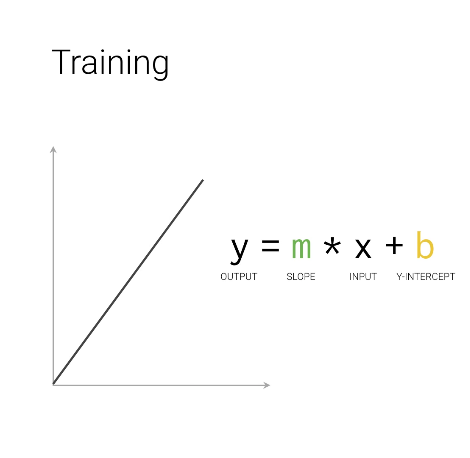
\includegraphics[height=5.5cm]{images/ml1_1.png}
\end{center}

On place les paramètres sur droite $d \equiv y = mx+b$ où
$$\begin{cases}x$ est l’entrée$ \\
m$ est la pente$ \\
b$ est l'ordonnée à l'origine$ \\
y$ est la valeur de $d$ en un point précis, c'est la sortie$
\end{cases}$$


Pour modifier la position de la droite, on joue sur les paramètres $m$ et $b$ ($m$ et $b$ sont les différentes valeurs des caractéristiques). Pour que le système puisse assimiler toute l’information, on utilise des matrices. 
La matrice des $m$ est la matrice des poids (\textit{weights}) et la matrice des $b$ est la matrice des biais (\textit{biases}). 

\begin{center}
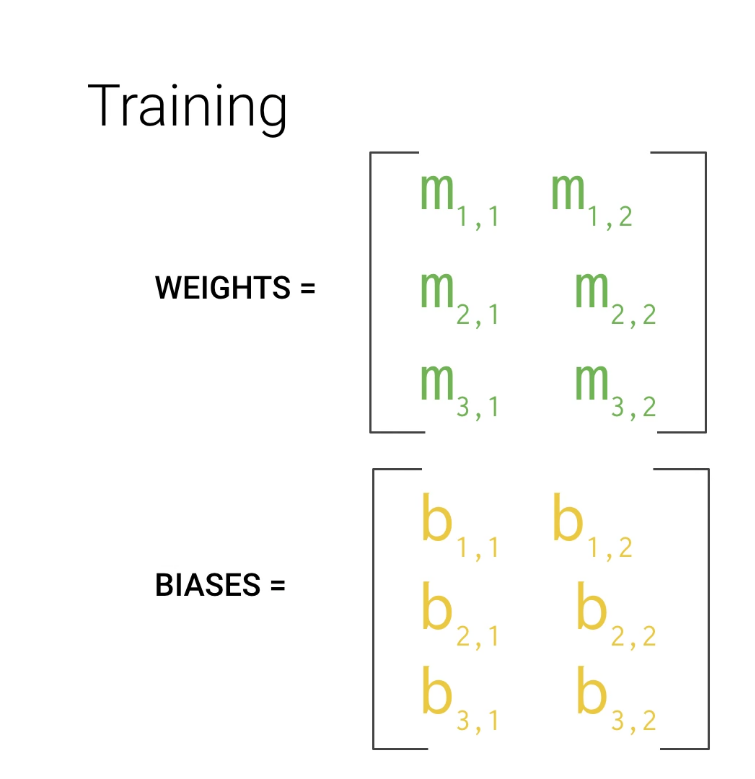
\includegraphics[height=7.5cm]{images/ml1_2.png}
\end{center}

Il faut un système avec tous les paramètres $m$ et tous les paramètres $b$ et le but est de, en faisant varier les paramètres, entrainer le système à reconnaitre et à faire des prédictions de plus en plus fiable.

\item Evalutation : après l’entrainement, une évaluation du système avec des nouvelles données nous aide à voir le pourcentage de fiabilité du module.

\item Paramètre et hyperparamètre : ce sont deux types de paramètre. Ces paramètres expriment les propriétés de «niveau supérieur» du modèle telles que la complexité et la rapidité d'apprentissage. Les hyperparamètres, ne pouvant pas être directement appris sur base de l'entrainement, sont généralement fixés avant-même que le processus d’apprentissage commence. De manière générale, on fixe la valeur de l’hyperparamètre, après avoir testé différentes valeurs de celui-ci et en décidant lesquels fonctionnent le mieux.

\item Prédiction : il ne reste plus qu’à faire tourner le système avec les données qui nous intéressent  pour obtenir la reconnaissance des différentes pièces monnaies. 
\end{enumerate}

\subsubsection{Différents type de machine learning}
\paragraph{Apprentissage supervisé}
L'apprentissage supervisé est la forme de machine learning la plus répandue. Elle consiste à entrainer l'algorithme sur des entrées $X$ dont on connait les sorties $Y$. Il y a eu donc au préalable une intervention d'un expert qui a lié les entrées $X$ et les sorties $Y$ entre elles.
\paragraph{Apprentissage non-supervisé}
L'apprentissage non-supervisé consiste à faire aucun lien entre les entrées et sorties. L'algorithme doit trouver par lui-même la strucure cachée entre les données. Ainsi, aucun expert n'est requis. Et la phase de prédiction est dès lors impossible : l'algorithme classe uniquement les données.
\paragraph{Apprentissage par renforcement}
Par ce dernier apprentissage, l'algorithme modifie son comportement au vu des observations et des résultats qu'il tire de ses expériences. Chaque nouvelle action de l'algorithme lui permet de connaître mieux son environnement et ainsi d'optimiser d'avantage son apprentissage.

\subsection{Transform\'ee de Hough}

\subsubsection{Introduction}
La transform\'ee (ou transformation) de Hough est une technique de reconnaissance de formes invent\'ee en 1962 par Paul Hough. \\
L'application la plus simple permet de d\'etecter les lignes/droites pr\'esentes dans une image mais des modifications peuvent \^etre apport\'ees \`a cette technique pour d\'etecter d'autres formes g\'eom\'etriques (cercles, ellipses...) : c'est la transform\'ee g\'en\'eralis\'ee de Hough d\'evelopp\'ee par Richard Duda et Peter Hart en 1972. \\
Cette technique est devenue un outil standard dans le domaine de la vision artificielle.

\subsubsection{Principe}
Le probl\`eme pos\'e est celui de la recherche et de la d\'etection de lignes qui seraient \'eventuellement pr\'esentes dans une image \`a analyser. Le principe de la transform\'ee de Hough est qu'il existe un nombre infini de lignes qui passent par un point, dont la seule diff\'erence est la pente a, l'orientation, l'angle... Le but de la transform\'ee est de d\'eterminer lesquelles de ces lignes sont les plus pr\'esentes dans l'image analys\'ee.
\begin{center}
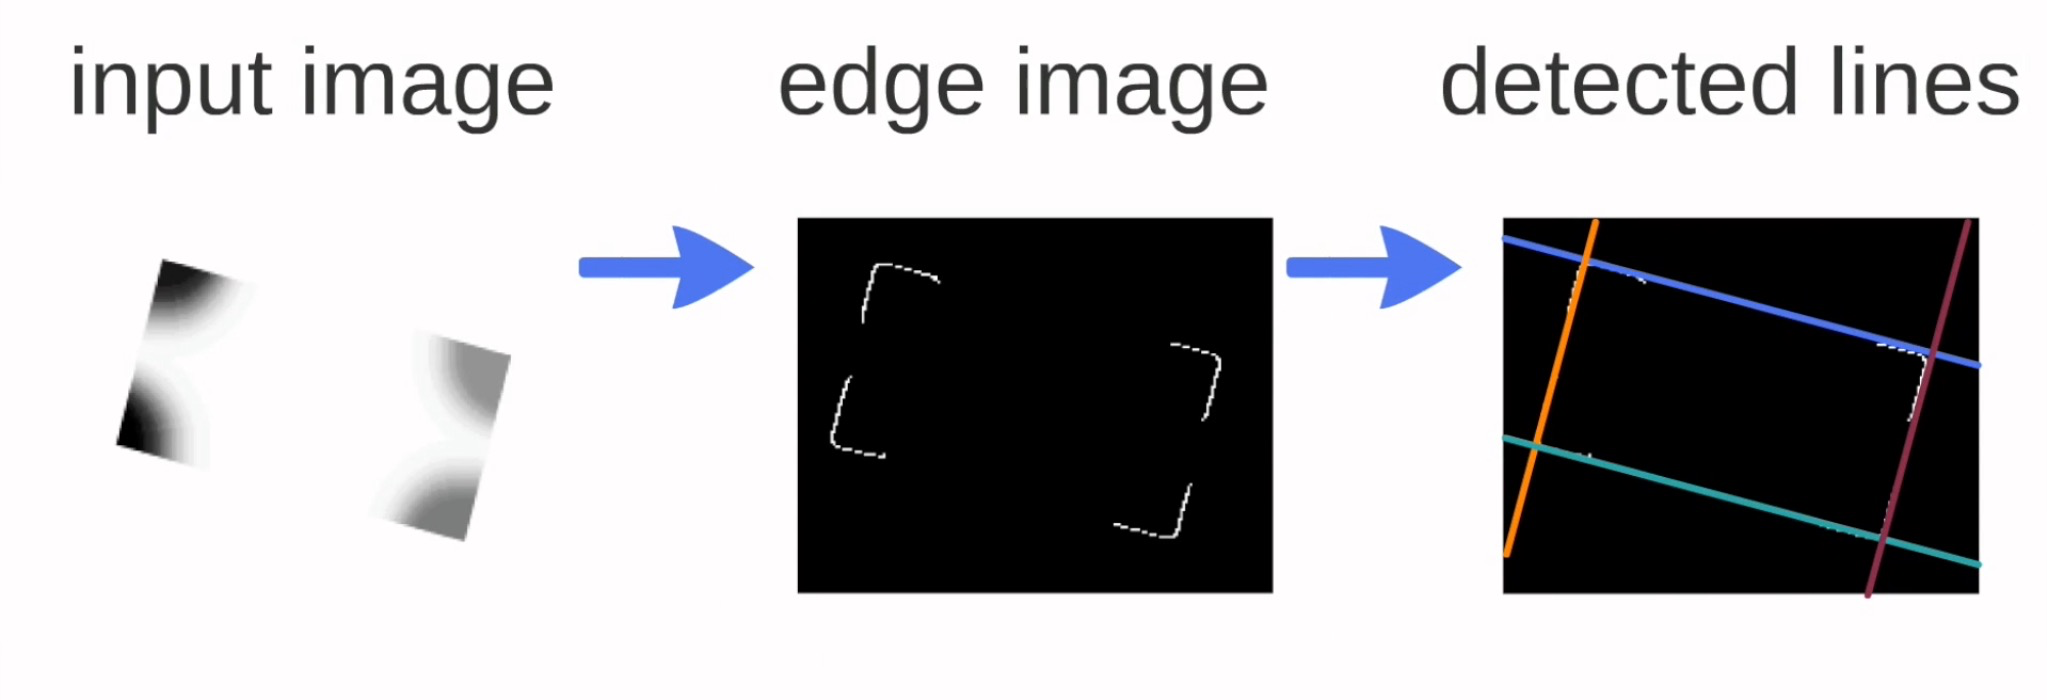
\includegraphics[height=4cm]{images/hough_1.png}
\end{center}

\subsubsection{Premi\`ere approche}

\paragraph{Repr\'esentation d'une droite}
La formule la plus simple repr\'esentant une droite dans le plan est son \'equation cart\'esienne et r\'eduite $y=ax+b$ (avec $a, b \in \mathbb{R}$) où
$$\begin{cases}
a$ est la pente de la droite$ \\
b$ est l'ordonn\'ee \`a l'origine$
\end{cases}$$

\begin{center}
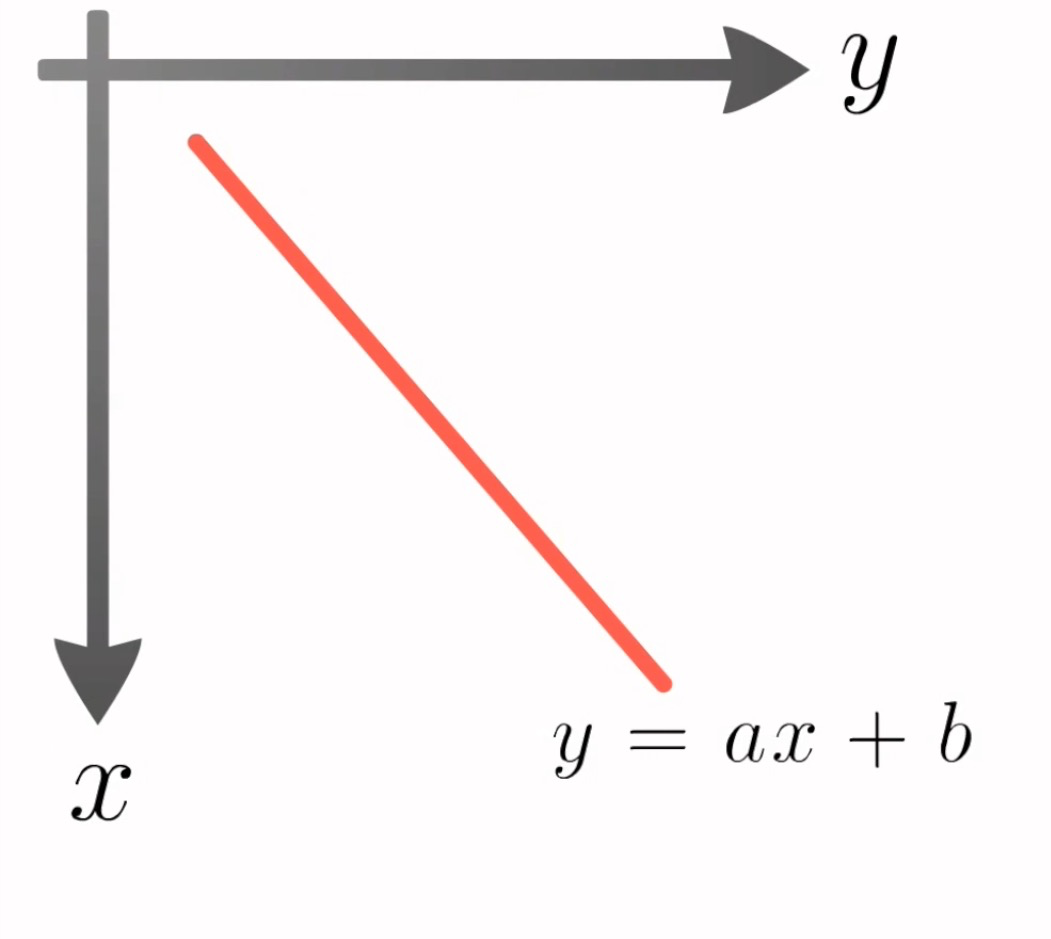
\includegraphics[height=3cm]{images/hough_2.png}
\end{center}
Toutes les droites passant par un point de coordonn\'ees $(x_1, y_1)$ fix\'ees ont la forme $y_1=ax_1+b$ pour diff\'erentes valeurs de $a$ et $b$. 
\begin{center}
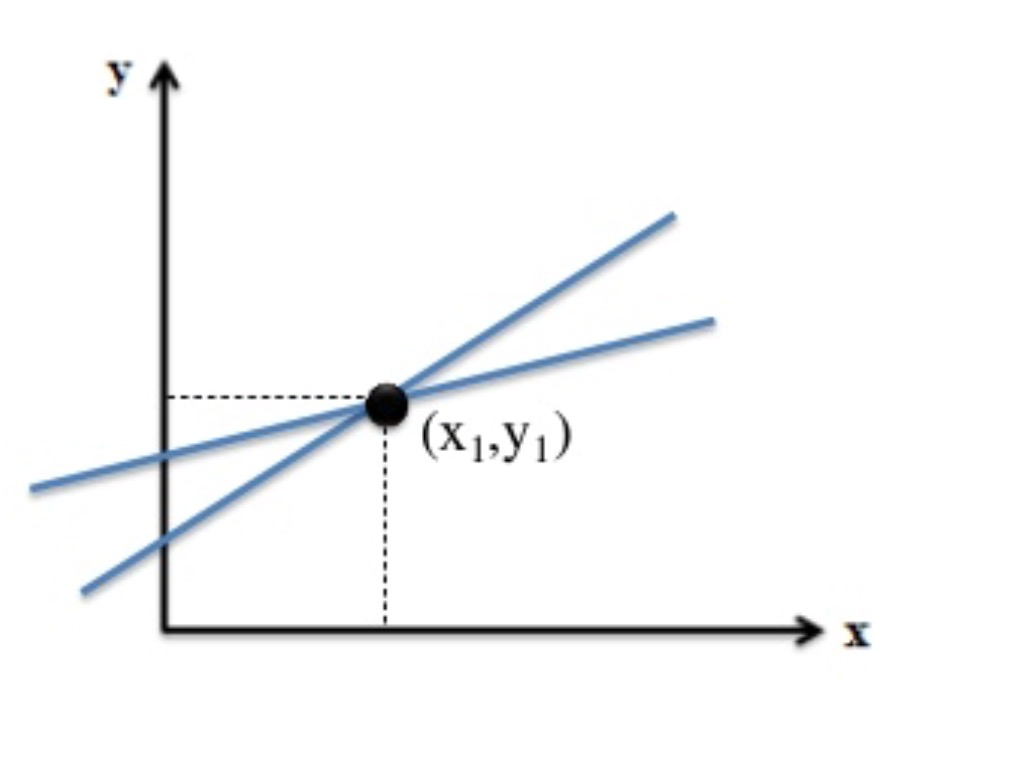
\includegraphics[height=3cm]{images/hough_8.png}
\end{center}

\paragraph{Principe d\'etaill\'e}
\subparagraph{}
On va changer le rep\`ere en rempla\c cant $x$ par $a$ et $y$ par $b$.
Chaque droite dans l'espace $(x, y)$ sera transform\'ee en un point dans l'espace $(a, b)$, espace de Hough.
Invers\'ement, chaque point dans l'espace $(x, y)$ sera transform\'e en une droite d'\'equation $b=-ax+y$ dans l'espace de Hough.
\begin{center}
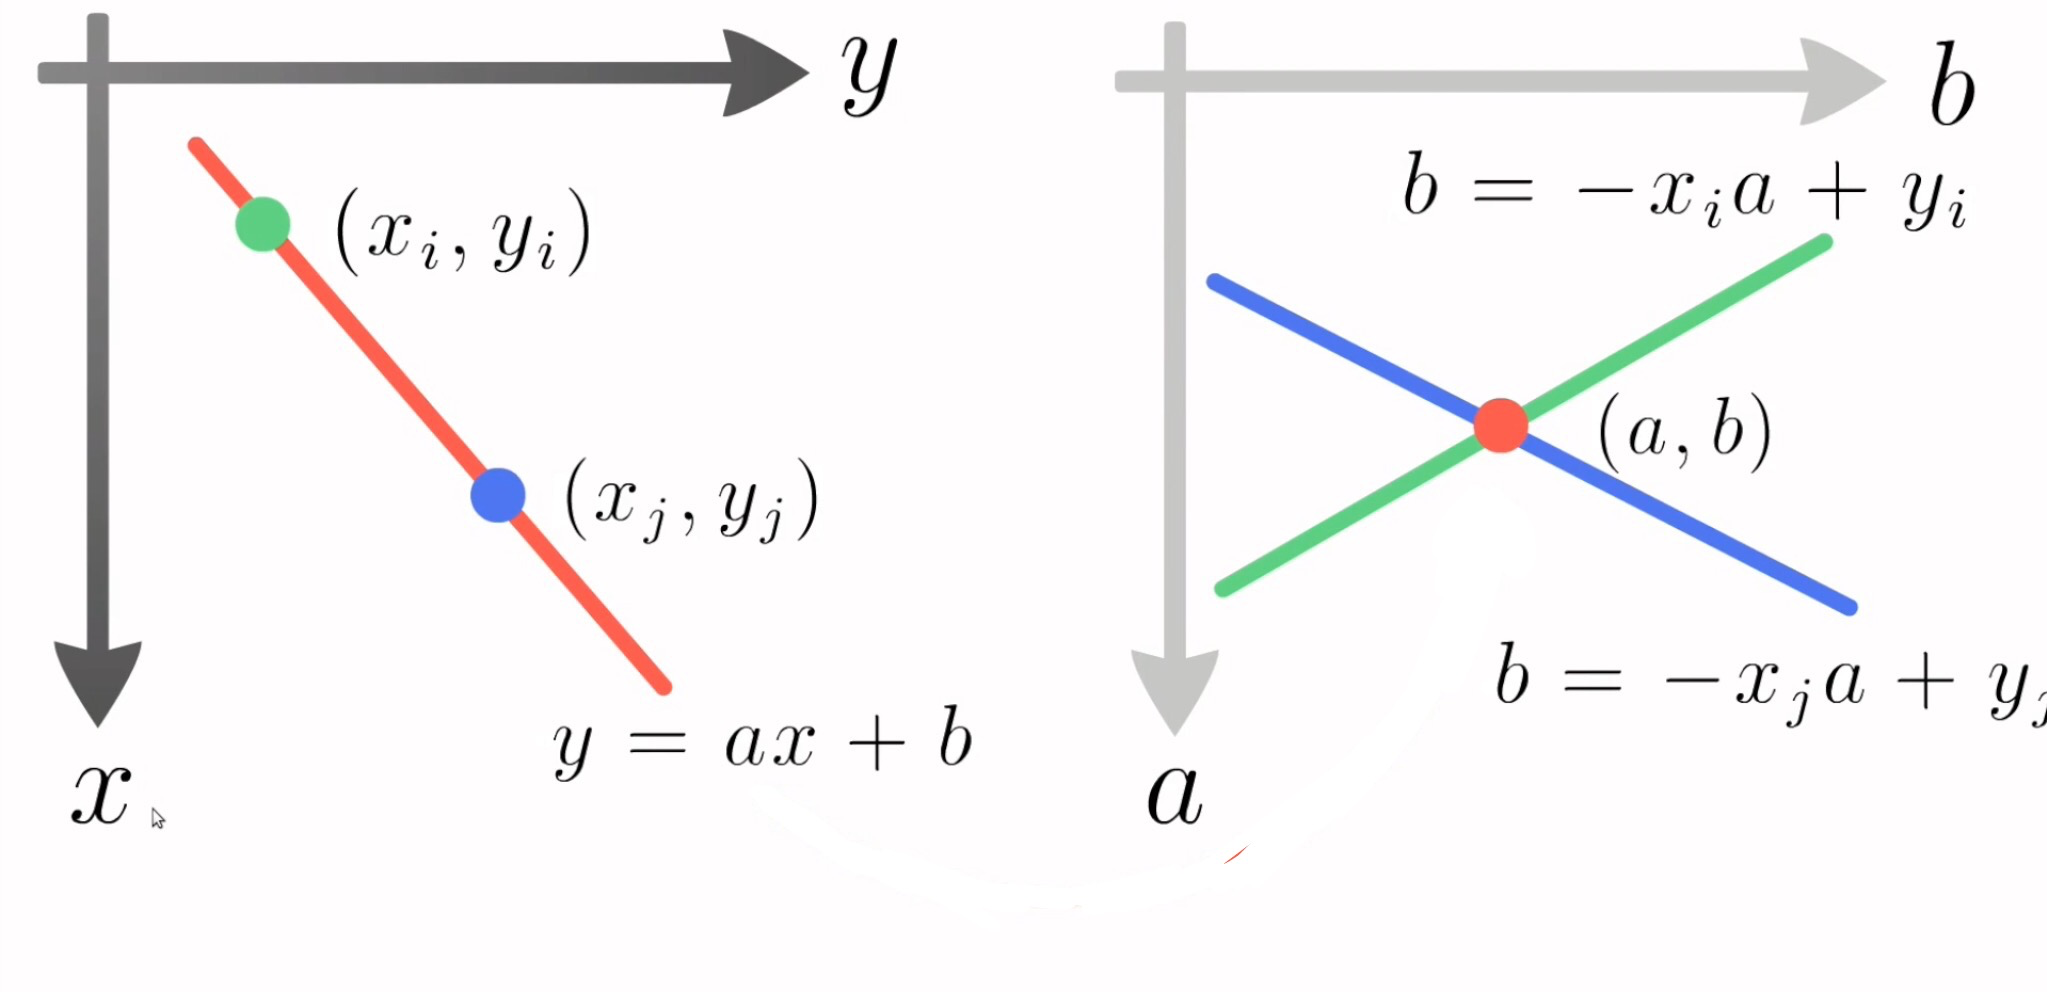
\includegraphics[height=3cm]{images/hough_3.png}
\end{center}
Pour un point $A$, toutes les droites passant par ce point correspondent \`a une seule droite $a$ dans l'espace de Hough.
Pour un point $B$, toutes les droites passant par ce point correspondent \`a une seule droite $b$ dans l'espace de Hough.
Ces $2$ faisceaux de droites dans l'espace $(x, y)$ ont en commun l'unique droite qui relie $A$ et $B$.
Cette droite correspond au point qui est l'intersubsection des $2$ droites $a$ et $b$.
Finalement, cette intersection contient les param\`etres de la droite recherch\'ee.

\subparagraph{}
Tous les points situ\'es sur une m\^eme droite $c$ dans l'espace $(x, y)$ sont repr\'esent\'es par des droites passant toutes par un m\^eme point $C$ dans l'espace de Hough.
Les coordonn\'ees de ce point $C(x_c, y_c)$ contiennent les param\`etres recherch\'es de la droite $c \equiv y=x_cx+y_c$. Afin de déterminer quelles droites sont les plus présentes, on utilise un accumulateur o\`u chaque point peut voter pour une droite particuli\`ere et les droites recevant le plus de votes sont conserv\'ees.
On ne va cependant pas d\'evelopper ce principe ici.

\subparagraph{}
Remarquons que la repr\'esentation $y=ax+b$ pose un probl\`eme pour les droites verticales.  Voil\`a pourquoi la repr\'esentation suivante, qui r\`egle ce probl\`eme, est la plus utilis\'ee.

\subsubsection{Approche trigonom\'etrique}

\paragraph{Repr\'esentation polaire d'une droite}
Une droite peut aussi \^etre repr\'esent\'ee par la formule $y\sin\theta+x\cos\theta=\rho$ (avec $\theta \in [-\pi/2 ; \pi/2]$ et $\rho \in [0 ; d]$ où $d$ est la longueur de la diagonale de l'image)  o\`u

$$\begin{cases}
\theta$ est l'angle entre l'axe $x$ et le vecteur $\vec\rho \\
\rho$ est la distance la plus courte entre l'origine du rep\`ere et la droite$
\end{cases}$$

\begin{center}
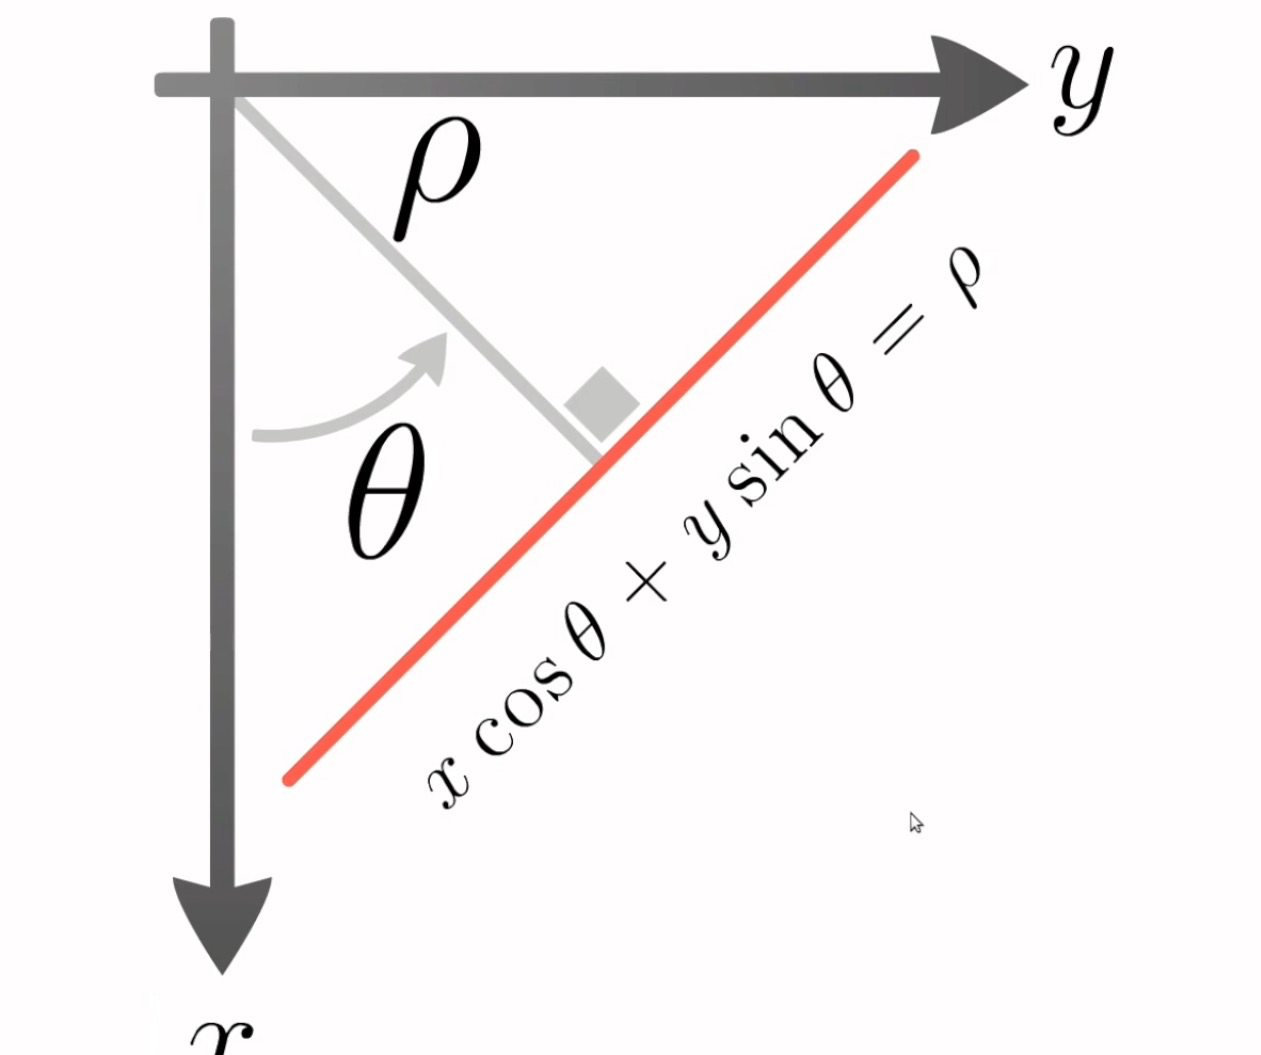
\includegraphics[height=3cm]{images/hough_4.png}
\end{center}

\paragraph{Principe d\'etaill\'e}
\subparagraph{}
On change \'egalement le rep\`ere en rempla\c cant $x$ par $\theta$ et $y$ par $\rho$.
Chaque droite dans l'espace $(x, y)$ est alors transform\'ee en un point dans l'espace $(\rho, \theta)$.
Chaque point dans l'espace $(x, y)$ est alors transform\'e en une courbe, une sinuso\"ide dans l'espace $(\rho, \theta)$.
Les points d'intersubsection des sinuso\"ides dans l'espace $(\rho, \theta)$ sont utilis\'es pour trouver les droites dans l'espace $(x, y)$.

\subparagraph{}
La transform\'ee de Hough fait ensuite appel \`a un algorithme qui regarde tous les points et imagine toutes les valeurs possibles pour $\rho$ et $\theta$.
On observe, dans l'espace $(\rho, \theta)$, des pics pour les valeurs qui reviennent le plus souvent et l'algorithme va d\'efinir les droites dans l'espace $(x, y)$ et donc les lignes d\'etect\'ees dans l'image.
\begin{center}
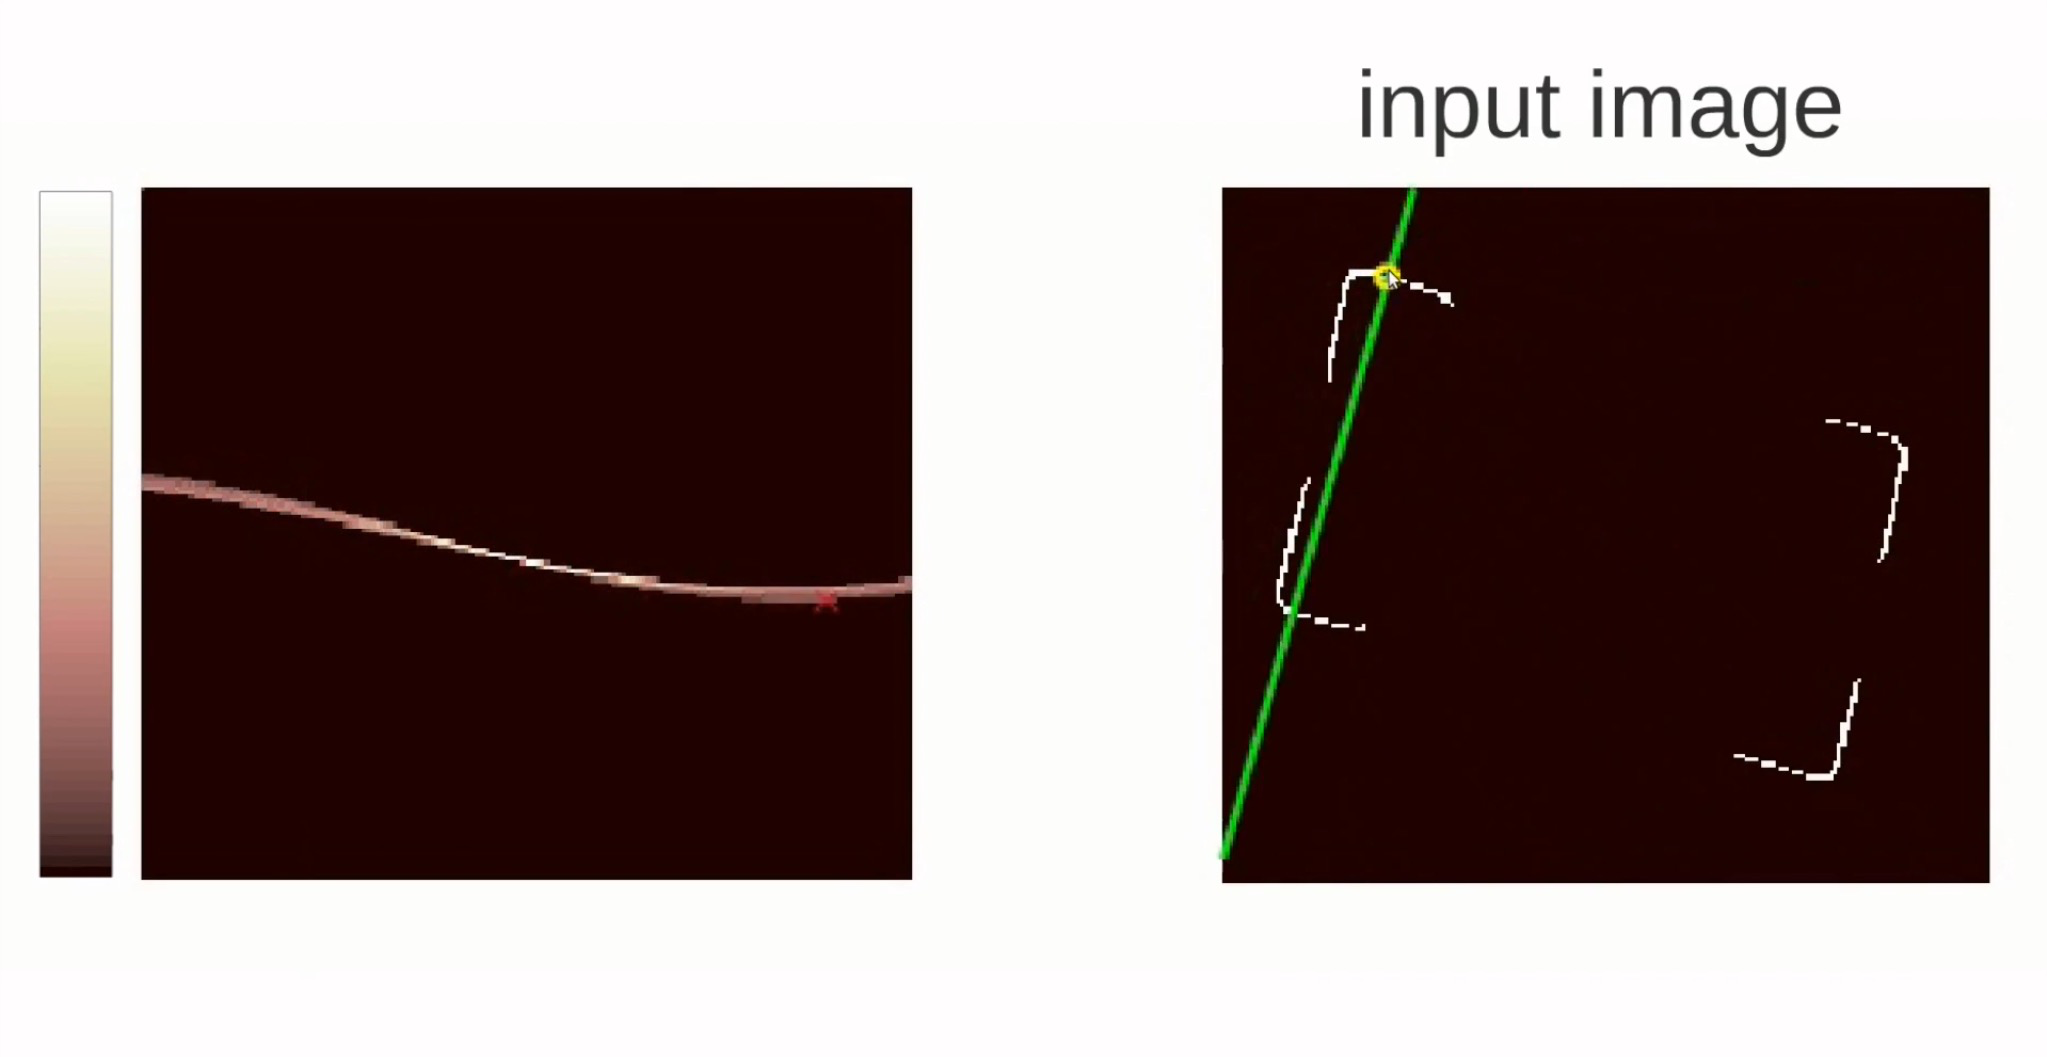
\includegraphics[height=3cm]{images/hough_5.png} \\
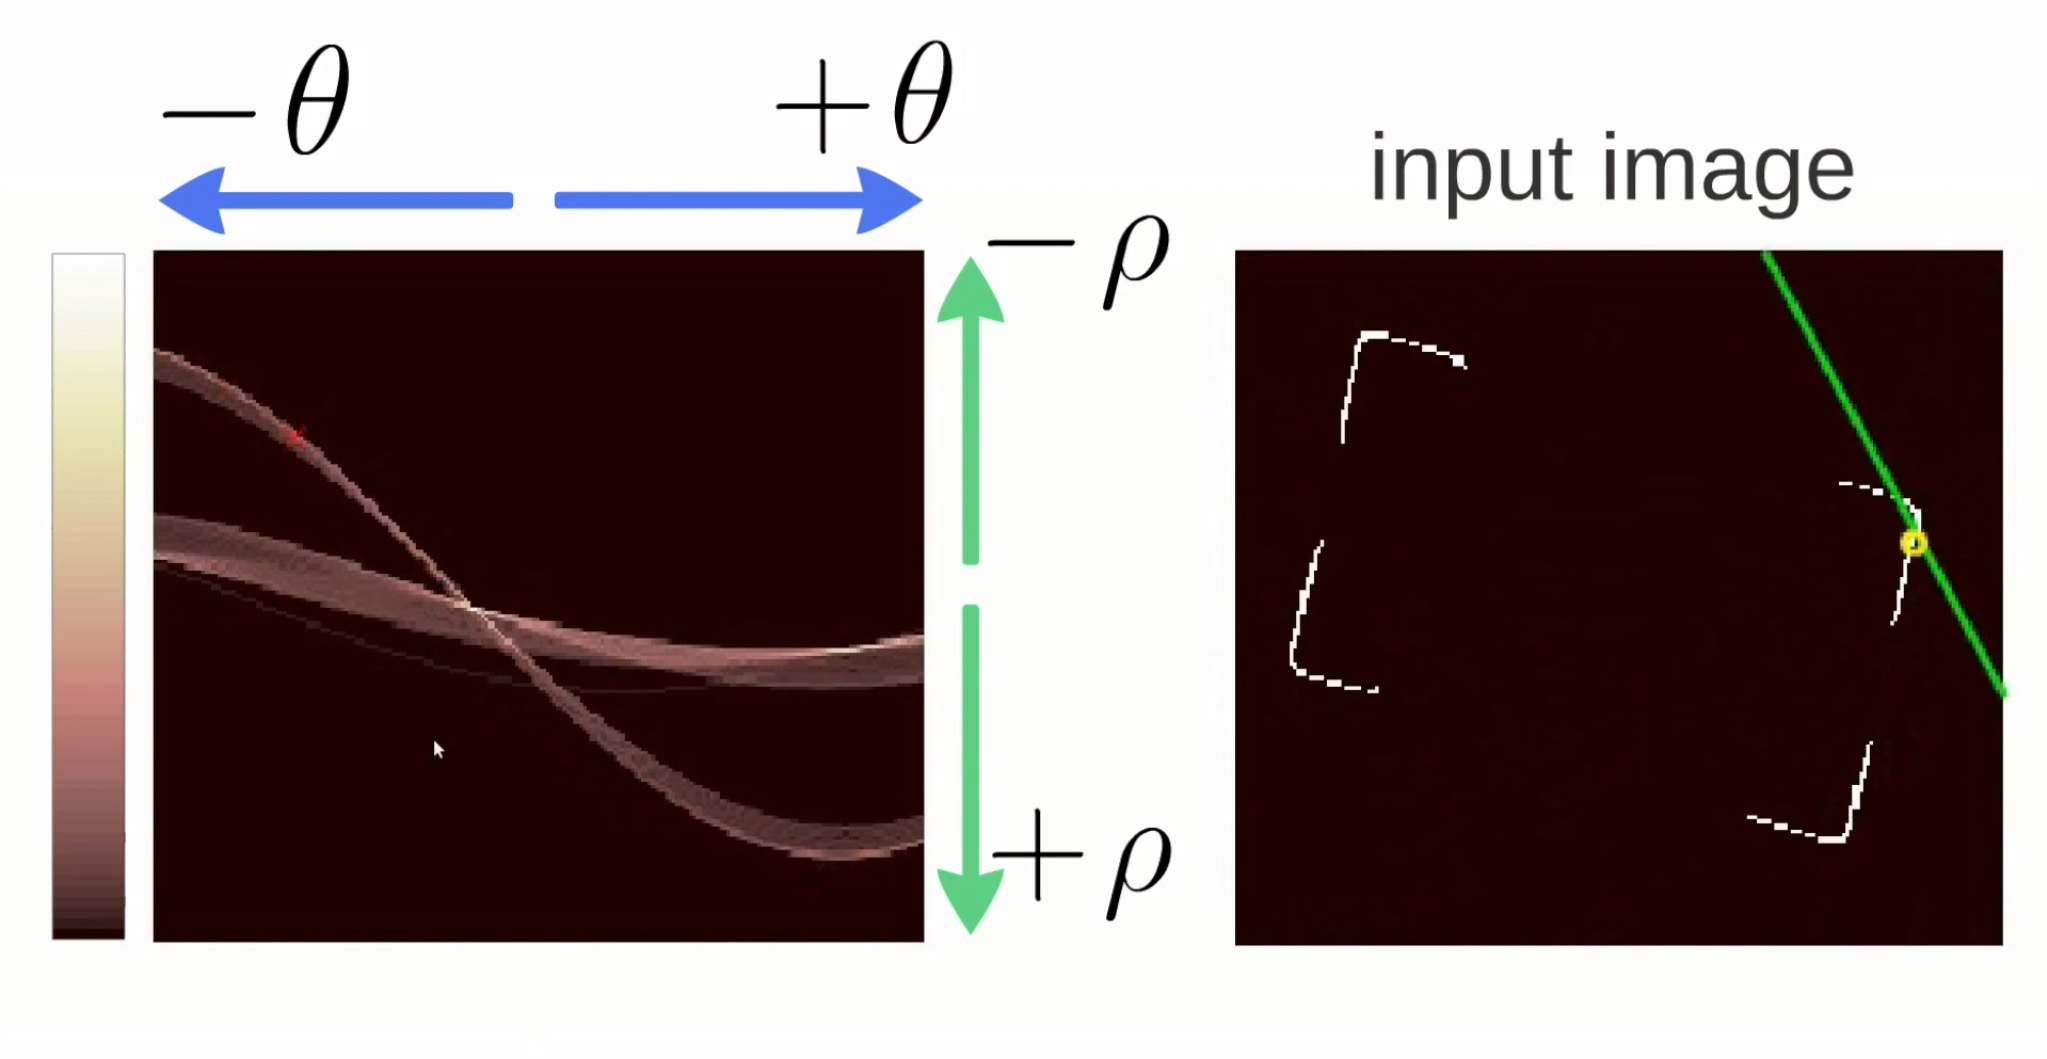
\includegraphics[height=3cm]{images/hough_6.png} \\ 
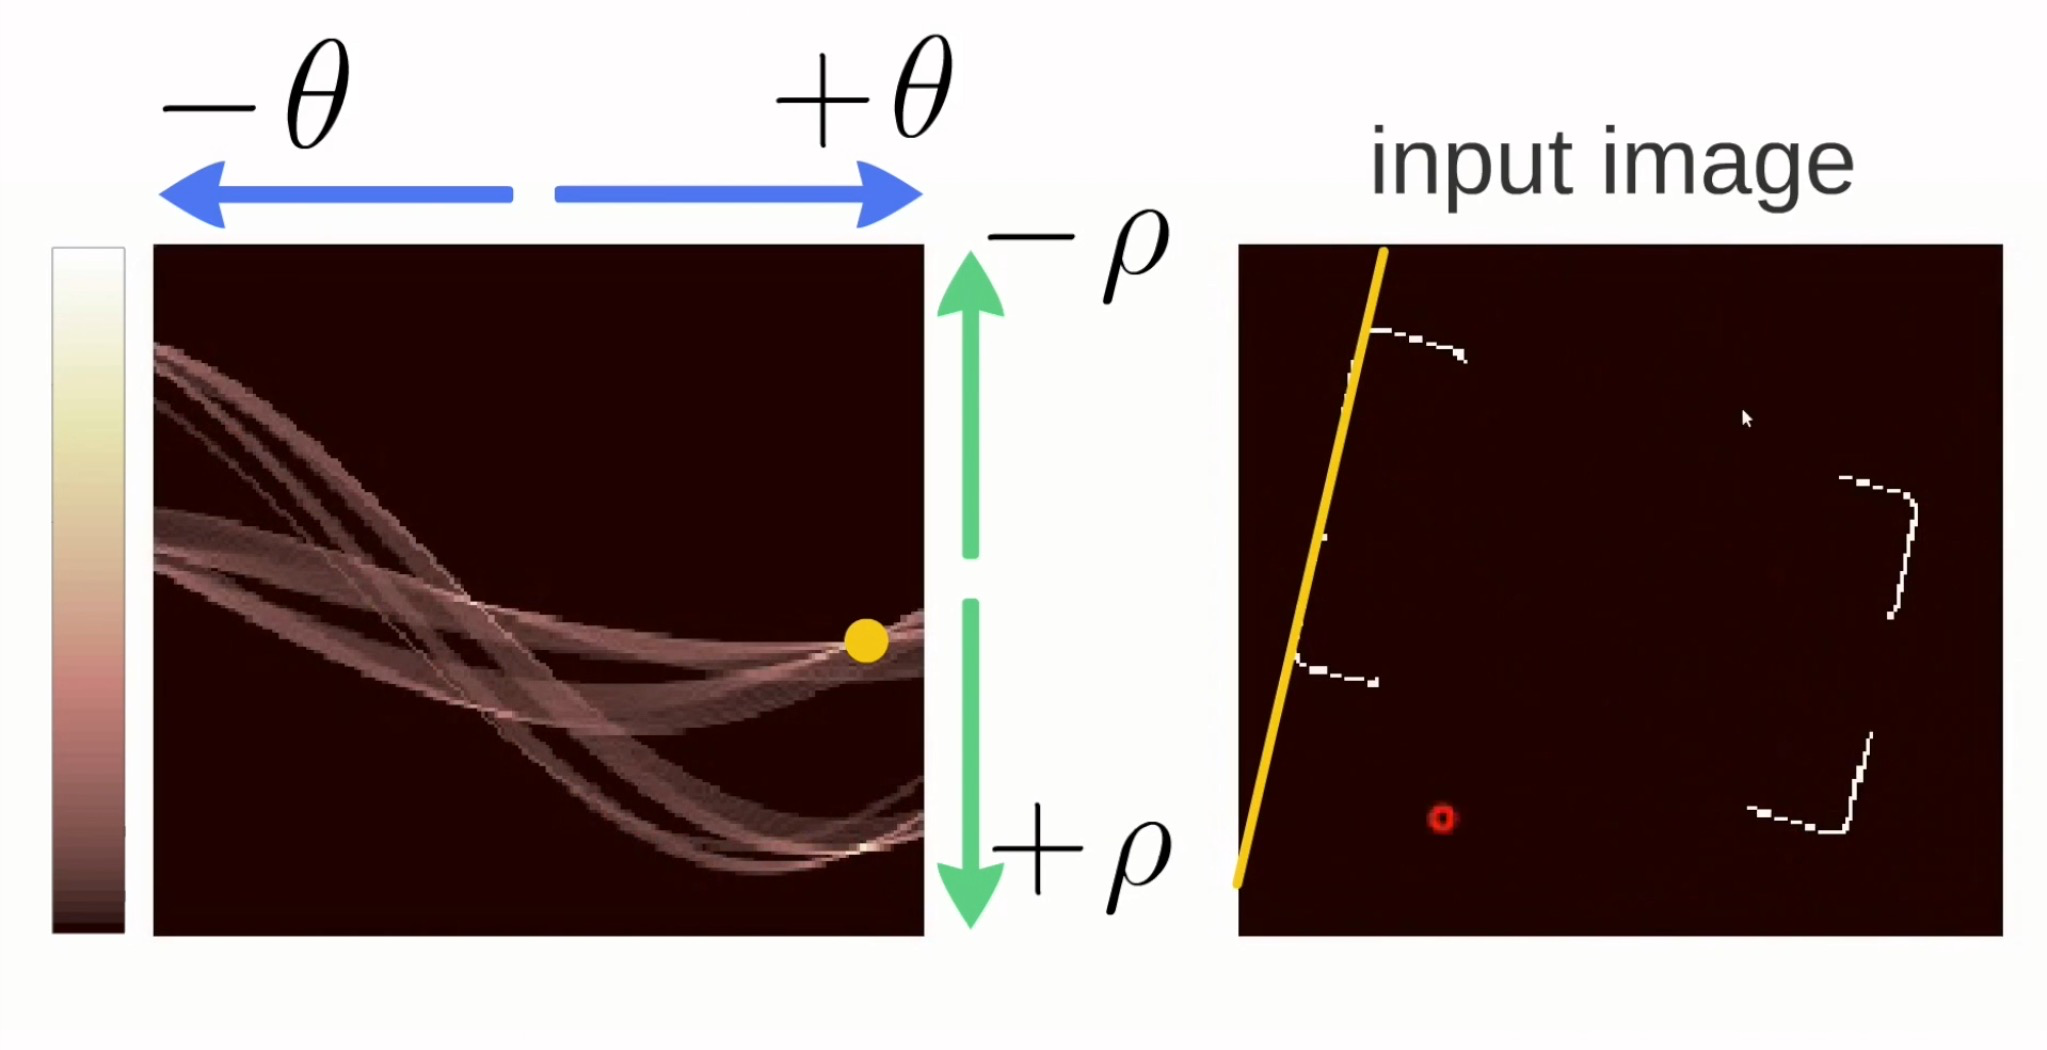
\includegraphics[height=3cm]{images/hough_7.png}
\end{center}

\subsubsection{Conclusion}
La transform\'ee de Hough est un outil efficace pour trouver les lignes dans une image. \\
Il existe d'autres transform\'ees de Hough pour extraire d'autres formes. \\
Elle est utilis\'ee dans plusieurs applications : d\'etection de routes dans les images prises par satellite, lecture de codes barres...

\subsection{Détection d'ensembles d'une même couleur} % TODO: Trouver un nouveau sous-titre
Une autre approche pour détecter des pièces de monnaie sur une image est d'exploiter le contraste entre les pièces elles-mêmes et le matériau sur lequel elles sont placées. Dans l'image suivante, par exemple, les pièces sont jaune ou rouge foncé alors que le fond est blanc.

\begin{center}
\includegraphics[width=0.5\linewidth]{images/manycoins.png}
\end{center}

Nous allons développer un algorithme permettant d'utiliser la couleur du fond pour isoler les pièces. Et nous allons l'appliquer à cette image afin d'en extraire les pièces.

\section{Un algorithme en profondeur}

\subparagraph{}
L'algorithme se décompose en $2$ passes principales, suivies de $2$ filtres heuristiques. Avant de parler de ces éléments, nous devons introduire du vocabulaire sur les graphes et présenter quelques algorithmes simples.

\subsection{Généralités sur les graphes}

Un graphe est un ensemble de points appelés \textit{sommets} (\textit{\textbf{v}ertices} en anglais) et de connections appelées \textit{arêtes} (\textit{\textbf{e}dges} en anglais). Voici par exemple un graphe de $6$ sommets et de $7$ arêtes:

\begin{center}
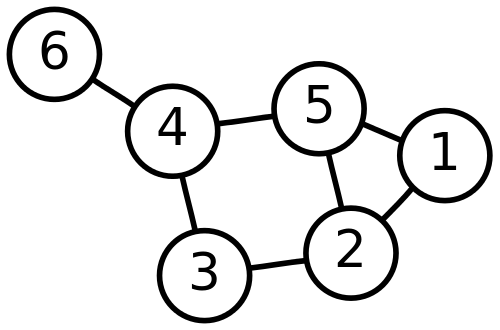
\includegraphics[width=0.5\linewidth]{images/graph.png}
\end{center}

Dans ce cas-ci, les points sont $1, 2, 3, 4, 5, 6$ et les connections sont \\ $(1,2),(1,5),(2,3),(2,5),(3,4),(4,5),(4,6)$. \\
D'un point de vue mathématique, le \textbf{g}raphe G peut se définir ainsi: 
$$\begin{array}{l}
G = (V, E), \\
V = \{1,2,3,4,5,6\}, \\
E = \{(1,2),(1,5),(2,3),(2,5),(3,4),(4,5),(4,6)\}.
\end{array}$$

% TODO: définir chemin, sommet adjacent

\subsection{Composantes connexes}
Le graphe ci-dessus est un exemple de graphe \textit{connexe}, c'est-à-dire un graph dont tout point est relié à tout point. Il existe aussi des graphes non connexes. Les différentes parties connexes du graphe sont alors appelées des \textit{composantes connexes}. Le graphe ci-dessous est ainsi composé de $3$ composantes connexes. Il est clair que le graphe est non connexe car le point $1$ n'est par exemple pas relié au point $3$.

\begin{center}
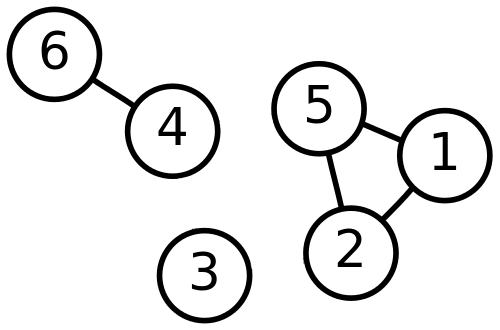
\includegraphics[width=0.5\linewidth]{images/3-components.png}
\end{center}

\subsection{Parcours d'un graphe}
\subparagraph{}
Voyons maintenant comment on peut détecter les différentes composantes connexes d'un graphe. Pour ce faire, commençons par remarquer la transitivité de la définition d'une composante connexe. En effet, s'il existe un chemin de $u$ à $v$ et de $u$ à $w$, il existe forcément un chemin allant de $v$ à $w$ et inversément. Il suffit en effet de partir de $v$, de se rendre à $u$ et de rejoindre $w$ depuis $u$. Cette propriété peut sembler anodine, mais elle affirme que pour détecter une composante connexe, il suffit de partir d'un sommet quelconque et de parcourir le graphe en catalogant tous les sommets atteignables.

\subparagraph{}
Un algorithme classique pour parcourir les graphes est le \textit{depth-first search} (DFS) ou encore \textit{parcours en profondeur}, appelé ainsi parce qu'il va aussi loin qu'il peut avant de revenir en arrière. \\
On part d'un sommet $u$. Si le sommet $u$ n'a pas encore été visité, on le marque comme visité. Ensuite, pour chaque sommet $v$ adjacent à $u$, on reprend l'algorithme récursivement. En C++, cela donne:

\lstinputlisting[caption=DFS]{src/simple-dfs.cpp}

\subparagraph{}
Cet algorithme ne parcourt qu'une seule composante connexe. Afin de détecter toutes les composantes connexes, on peut essayer de lancer l'algorithme depuis chaque sommet. Si l'algorithme n'a pas encore été lancé depuis un sommet $u$, c'est que $u$ appartient à une nouvelle composante connexe.

\lstinputlisting[caption=Composantes connexes]{src/simple-dfs-call.cpp}

\subparagraph{}
Ce code parcourt bien tous les sommets mais il ne permet toujours pas de déterminer la composante connexe d'un sommet donné. Réglons ce problème: plutôt que d'enregistrer si un sommet a été visité ou non, on peut directement enregistrer à quelle composante connexe il appartient.

\lstinputlisting[caption=Composantes connexes]{src/simple-cc-full.cpp}

\subsection{Première passe: ensembles de couleur}
\subparagraph{}
Appliquons maintenant ces idées à l'image. Pour ce faire, il faut savoir qu'une image est essentiellement une matrice de pixels, chacun composé de trois composantes $(r, g, b)$ (red, green, blue) avec $r, g, b$ discrets $\in [0, 255]$. Nous allons donc utiliser la structure de graphe implicite de cette matrice en prenant comme sommets les différents pixels et en stipulant qu'un pixel $(i, j)$ est adjacent aux pixels ${(i, j+1), (i, j-1), (i+1, j), (i-1, j)}$. Si nous calculons maintenant les composantes connexes de ce graphe, nous obtiendrons une unique composante contenant tout le graphe. C'est normal, le graphe est connexe d'après notre définition et nous n'avons d'ailleurs pas prix en compte les couleurs des pixels. Afin de pouvoir détecter des composantes connexes, nous aimerions isoler les zones de couleurs différentes. Nous devons donc connecter les pixels adjacents de couleurs très proches par des arêtes.

\subparagraph{}
Nous cherchons donc une fonction $f$ prenant deux pixels $p (r, g, b)$ et $p' (r', g', b')$ comme arguments et renvoyant $1$ ou $0$ selon que leurs couleurs sont proches ou non. C'est l'étape cruciale de l'algorithme. En effet, une fonction mal choisie ne permettra pas de détecter de bonnes composantes connexes. Cependant, comme nous allons le voir dans ce qui va suivre, nous voulons uniquement détecter la composante connexe la plus grande, c'est-à-dire celle du fond sur lequel les pièces reposent. Nous allons donc nous contenter d'une fonction prenant la plus petite différence absolue entre chaque paire de composantes correspondantes. En pratique, cela donne:
$$f(p, p') = \left\{\begin{array}{ll} 1 & \text{si } max(|r-r'|, |g-g'|, |b-b'|) \le s \\ 0 & \text{sinon}\end{array}\right\}$$
où $s$ est un paramètre fixé au début de l'algorithme. La lettre $s$ a été choisie pour le terme anglais \textit{sharpness} et nous allons l'appeler coefficient de finesse. Pour de faibles valeurs de $s$, beaucoup de composantes connexes seront détectée. Si $s$ vaut $0$, chaque pixel sera une composante connexe. Pour de grandes valeurs de $s$, moins de composantes connexes seront identifiées. Si $s$ vaut $255$ ou plus, l'image ne sera qu'une grande composante connexe.

\subparagraph{}
La valeur à choisir en pratique dépend principalement de la résolution de l'image. En effet, les images à très haute résolution comme celle des pièces de monnaie plus haut (environ $3000$x$4000$ pixels) nécessitent de très faibles valeurs de $s$ à cause de la diffusion de la lumière alors qu'il convient de choisir des valeurs plus hautes pour des résolutions plus faible afin de s'assurer que le fond est bien une unique composante connexe. Voyons donc ce qui se passe pour $s=2$ (des couleurs aléatoires ont été choisies pour faciliter la visualisation des composantes connexes):

\begin{center}
\includegraphics[width=0.4\linewidth]{images/15coins/manycoins.png}
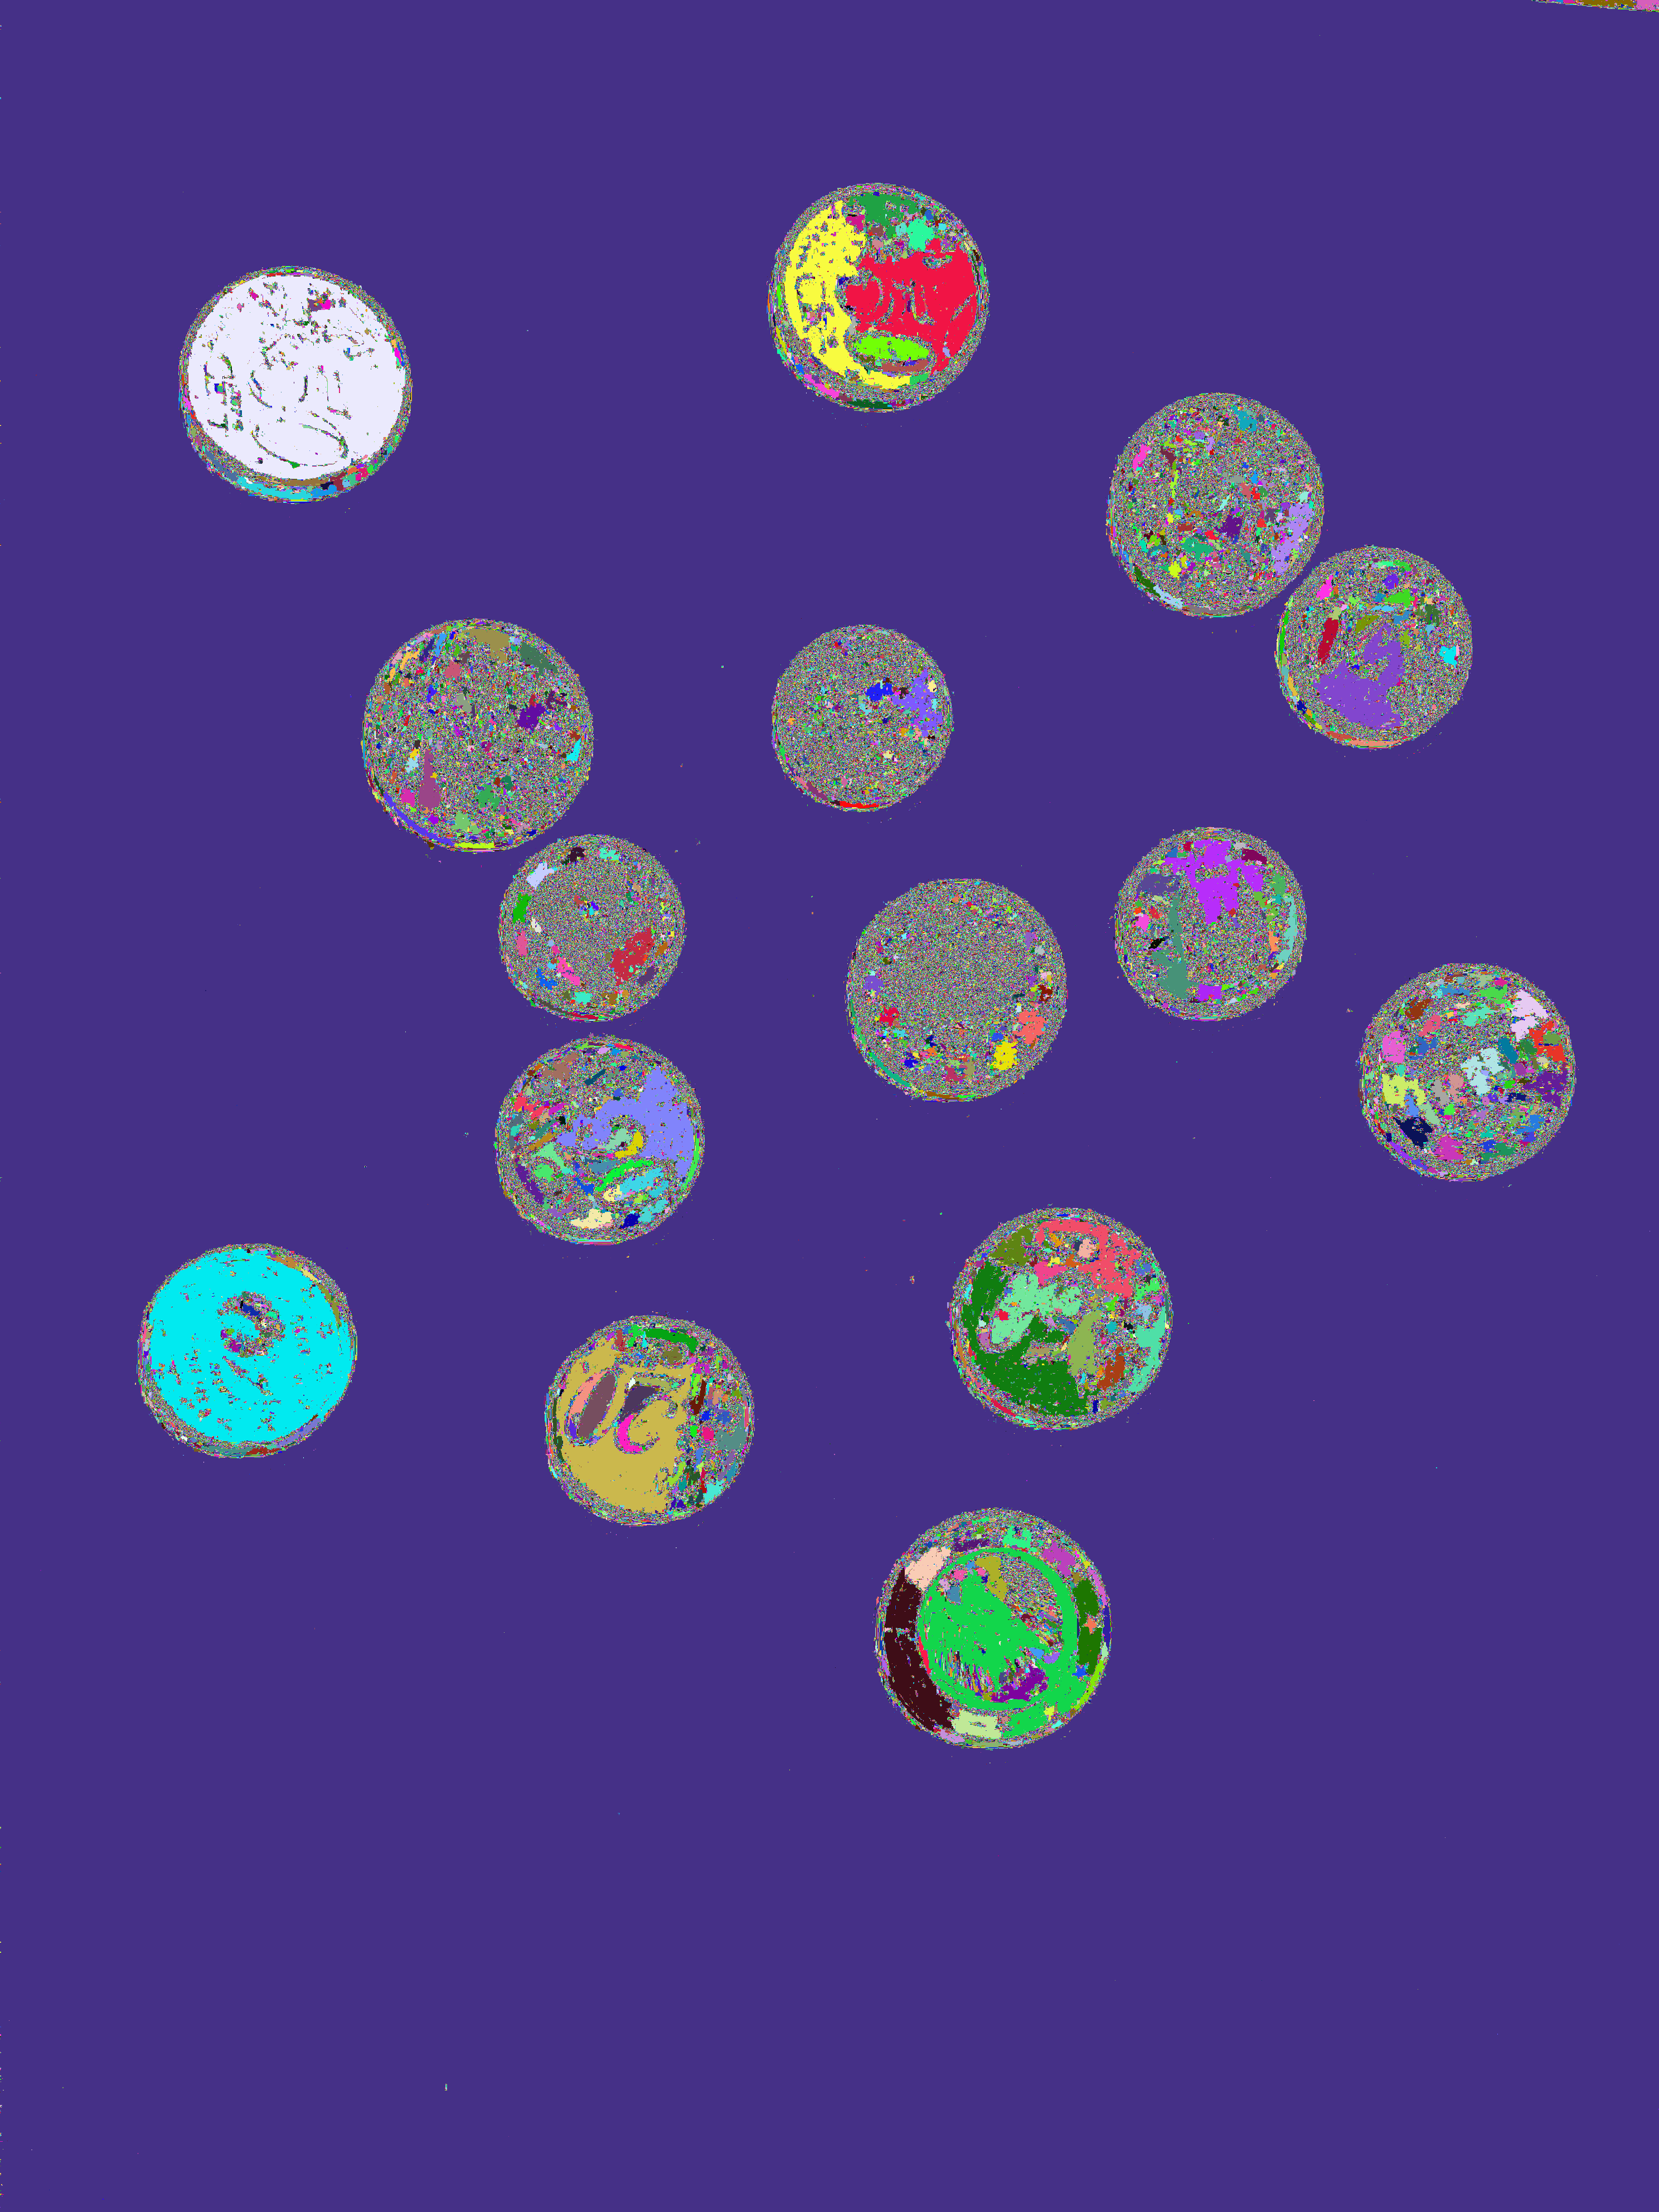
\includegraphics[width=0.4\linewidth]{images/15coins/out_manycolors.png}
\end{center}

Remarquons que le fond de l'image est correctement détecté, et c'est tout ce qui importe. Nous allons maintenant voir comment exploiter cette information pour compter le nombre de pièces.

\subsection{Deuxième passe: pièces de monnaie}
\subparagraph{}
Une fois que nous avons réussi à détecter le fond, nous pouvons séparer le graphe en deux parties: le fond et les pièces. Ceci peut être fait avec un algorithme trivial que nous ne détaillerons pas ici. Voici le résultat que l'on obtient:

\begin{center}
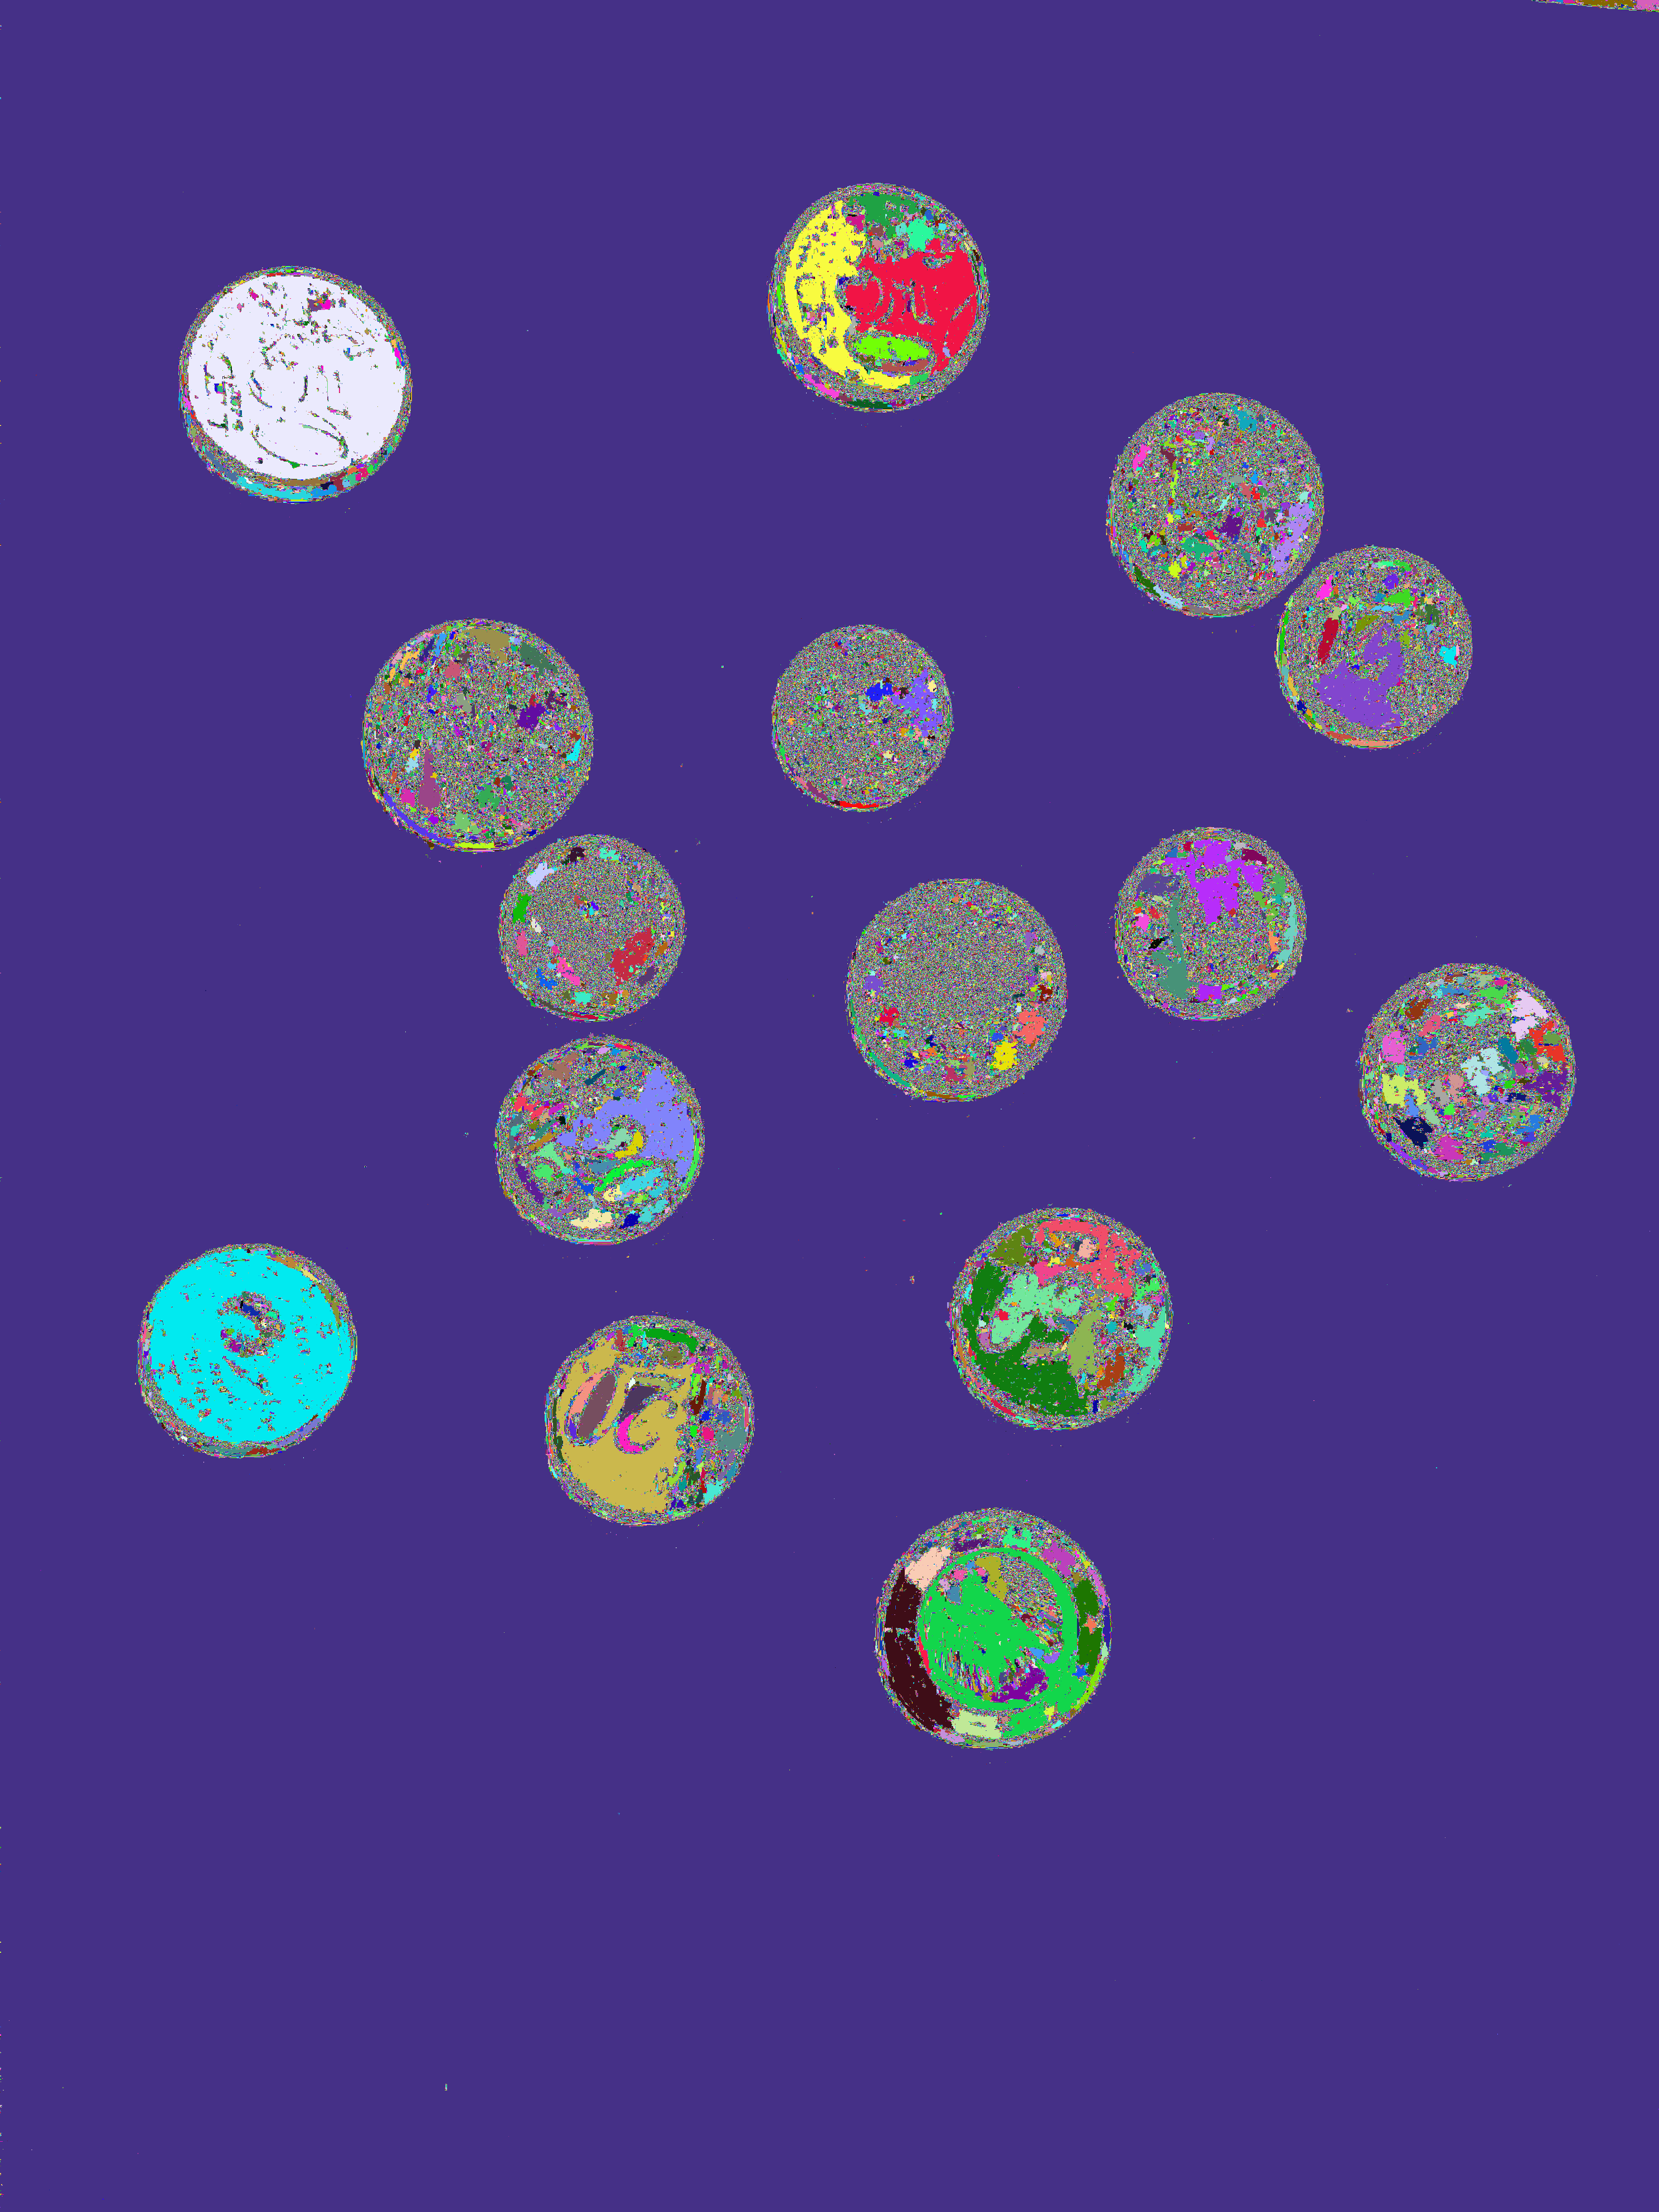
\includegraphics[width=0.4\linewidth]{images/15coins/out_manycolors.png}

\includegraphics[width=0.4\linewidth]{images/15coins/out_2colors.png}
\end{center}

\subparagraph{}
Maintenant, il ne reste plus qu'à détecter les pièces individuelles. Pour ce faire, il suffit calculer les composantes connexes du sous-graphe contenant les pièces, toujours avec un DFS. Pour ce faire, nous connectons les pixels adjacents s'ils appartiennent au même sous-graphe. Nous ne détaillons pas le code mais une version commentée se trouve en annexe. Nous n'accordons alors plus aucune importance à la couleur, la distinction entre le fond et les pièces ayant déjà été faite par la première passe. Le résultat obtenu est alors le suivant. De nouveau, des couleurs générées aléatoirement ont été utilisées pour aider à la visualisation:

\begin{center}

\includegraphics[width=0.4\linewidth]{images/15coins/out_2colors.png}

\includegraphics[width=0.4\linewidth]{images/15coins/out_chunks.png}
\end{center}

\subparagraph{}
C'est bien le résultat attendu, il suffit maintenant de compter le nombre de composantes connexes détectées parmi les pièces. Sur cette image, la réponse est évidemment... $1202$ !? L'image a l'air correcte à priori, comment se fait-il que l'algorithme détecte $1202$ pièces et non $15$ ? Une analyse détaillée de l'image révèle de toutes petites taches de couleur et lorsqu'on demande au programme d'afficher la taille des différentes composantes connexes on se rend compte que certaines ont une taille de $20$ pixels ou moins.

\subsection{Filtrage heuristique}
\subparagraph{}
Afin de déterminer quelles composantes connexes correspondent ou non à des pièces de monnaie, nous allons appliquer deux heuristiques. Premièrement, nous pouvons éliminer les composantes connexes d'une taille en pixels inférieure à $t\%$ de l'image, avec $t$ que nous appellerons coefficient de tolérance. Une valeur de $t=0.1$ fonctionne assez bien. Cela peut sembler peu mais pour une image de $12000000$ pixels, cela veut dire que les pièces doivent faire au moins $1200$ pixels, ce qui n'est pas négligeable. Avec cette modification, notre algorithme détecte correctement les $15$ pièces de monnaie.

\subparagraph{}
Deuxièmement, nous pouvons éliminer les composantes connexes qui n'ont pas la forme d'une ellipse. Bien qu'il n'ait pas fallu recourir à cette option pour cette image-ci, cela se révèle souvent nécessaire en pratique. Nous avons par exemple essayé d'appliquer notre algorithme à l'image ci-dessous. Le résultat est assez clair:

\begin{center}
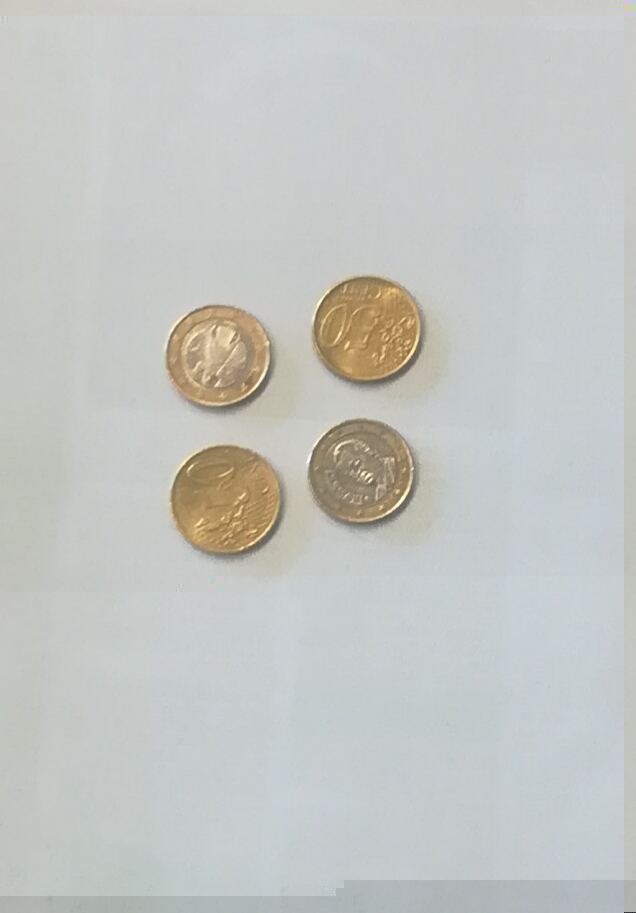
\includegraphics[width=0.4\linewidth]{images/4coins/img3.png}

\includegraphics[width=0.4\linewidth]{images/4coins/out_chunks.png}
\end{center}

Une approximation qui fonctionne assez bien en pratique est de calculer les valeurs minimale et maximale de $x$ et de $y$ pour tous les points appartenant à une composante connexe donnée. Nous pouvons alors calculer une approximation de l'aire sur base de ces valeurs en partant du principe que la forme repérée est une ellipse:
$$A = \frac{\pi}{4}\cdot |x_{min} - x_{max}|\cdot|y_{min} - y_{max}|$$.
Une fois cette aire calculée, nous pouvons comparer cette valeur à la taille en pixels de la composante connexe et nous assurer que l'erreur est bien inférieure à un certain pourcentage. Nous avons choisi $20\%$ mais une valeur plus faible aurait sans doute fait l'affaire.

\subsection{Complexité}
\subparagraph{}
La complexité d'un algorithme est définie comme la quantité de ressources (temps ou mémoire) nécessaire à son exécution. La notation $\mathcal O(\ldots)$ exprime la complexité asymptotique d'un algorithme dans le pire cas, où $\ldots$ est fonction d'un certain nombre de paramètres.

\subparagraph{}
Si nous prenons $w$ la largeur de l'image à analyser et $h$ sa hauteur, notre algorithme tourne en un temps $\mathcal O(wh)$. Posons $n = wh$ par simplicité. Chacun des DFS prend $\mathcal O(n + 4n) = \mathcal O(n)$. En effet, chaque sommet est visité une fois ($\mathcal O(n)$) et pour chaque sommet il faut tester les $4$ potentiels sommets adjacents ($\mathcal O(4n)$). Les heuristiques sont aussi en $\mathcal O(n)$ car elles nécessitent de parcourir tous les pixels exactement une fois. Notre algorithme tourne donc en $\mathcal O(n)$ et il est trivial de constater qu'il utilise $\mathcal O(n)$ en mémoire. Il est d'ailleurs impossible d'obtenir une complexité inférieure à partir du moment où on souhaite lire toute l'image, car la lecture prend au moins $\mathcal O(n)$ en temps et en mémoire. La partie la plus lente de notre programme est sans doute le chargement et la sauvegarde des images, car la bibliothèque utilisée pour ça doit suivre des algorithmes bien plus compliqués pour décoder et surtout encoder efficacement l'image. Pour garantir une complexité de $\mathcal O(n)$, nous pourrions utiliser un format de fichier non compressé comme les \textit{bitmaps} (.bmp) mais cela ne semble pas nécessaire en pratique et nous ne l'avons donc pas fait.

\subsection*{Conclusion}
\addcontentsline{toc}{section}{Conclusion}
Nous avons donc parlé de l'histoire de l'intelligence artificielle. Nous avons ensuite considéré plusieurs techniques pour résoudre le problème de la reconnaissance de pièces de monnaie. Finalement, nous avons développé un algorithme en particulier et nous avons déterminé que cet algorithme est très efficace: il a un temps d'exécution et une utilisation de mémoire optimaux et produit de bons résultats. Cerise sur le gâteau, nous proposons en annexe une piste d'amélioration afin de compter la valeur exacte de chacune des pièce.

\appendix

\section{Détection de la valeur des pièces}
\subsection{Détection de la figure des pièces}
Afin de détecter la valeur exacte de chaque pièce, nous pourrions maintenir une liste des différents symboles apparaissant sur les pièces de monnaie couramment utilisées dans le monde et voir duquel de ces symboles s'approchent le plus ceux des pièces détectées. Pour ce faire, nous pourrions prendre les valeurs des pixels le long de cercles pris à intervalles réguliers. Par exemple, nous pourrions décider de prendre $10$ cercles concentriques de rayons d'une longueur de $10\%, 20\%, \ldots, 100\%$ du rayon de chacune des pièces et de parcourir les pixels qui s'y trouvent. Nous pourrions ainsi comparer le signal obtenu et déterminer à quel symbole correspond une pièce de monnaie donnée en utilisant par exemple la méthode des moindres carrés. Malheureusement, cet algorithme ne tient pas compte de la rotation des pièces et garder traces de toutes les pièces de monnaie en usage dans tout le monde à tous les angles possibles ne semble pas faisable.

\subsection{Problème de la rotation}
Il existe une solution théorique relativement simple à ce problème. Il suffit en effet d'appliquer la transformée de Fourier à chacun des signaux et d'éliminer ensuite le déphasage afin d'aligner les différents signaux obtenus avant de reprendre l'algorithme.

\subsection{Caveat emptor}
Estimant que ces améliorations sortent de l'ampleur de notre TFE, nous n'avons pas creusé ces idées et nous ne les avons pas implémentées. Nous n'avons donc pas pu vérifier l'efficacité de l'algorithme suggéré ci-dessus et nous sommes peut-être passés à côté de certains problèmes essentiels avec cette nouvelle méthode. Bien qu'elle semble fonctionner d'un point de vue théorique, elle est donc à prendre avec des pincettes.

\section{Code de l'algorithme}
Voici le code que nous avons utilisé afin de compter le nombre de pièces de monnaie et de générer les différentes images présentées plus haut. Il nécessite la bibliothèque \textit{CImg}, elle-même faisant usage de $\textit{libpng}$ et de $\textit{libjpeg}$. Ce code compile sous Debian avec les options suivantes:
\begin{lstlisting}
g++ -pthread -lpng -ljpeg -lX11 -std=gnu+14 main.cpp
\end{lstlisting}

\lstinputlisting[caption=Notre algorithme]{src/program/main.cpp}

\section{Bibliographie}

\subsection{Livres}
\sloppy
\begin{itemize}
\item Rafael C. Gonzalez et Richard E. Woods. (2008). \textit{Digital Image Processing - Third Edition}. Pearson.
\end{itemize}

\subsection{Articles}
\sloppy
\begin{itemize}
\item Yosra Hasnaoui, Balkiss Hamad et Khaled Fayala. \textit{Détection des droites par la transformée de Hough}. École Supérieure des Sciences et Techniques de Tunis.
\end{itemize}

\subsection{Internet}
%\small{
\begin{itemize}

\sloppy
\item \url{https://www.quora.com/What-are-hyperparameters-in-machine-learning}.
\item \url{https://www.lesechos.fr/idees-debats/cercle/cercle-161999-demystifier-la-machine-learning-2038392.php}.
\item \url{https://www.youtube.com/watch?v=nKW8Ndu7Mjw}.
\item \url{https://www.youtube.com/watch?v=trWrEWfhTVg}.
\item \url{https://www.youtube.com/watch?v=h0e2HAPTGF4}.
\item \url{https://openclassrooms.com/courses/initiez-vous-au-machine-learning/qu-est-ce-que-le-machine-learning}.
\item \url{https://www.youtube.com/watch?v=trWrEWfhTVg}.
\item \url{https://fr.wikipedia.org/wiki/Apprentissage_automatique}.
\item \url{https://openclassrooms.com/courses/initiez-vous-au-machine-learning/qu-est-ce-que-le-machine-learning}.
\item \url{https://www.quantmetry.com/single-post/2015/10/28/Une-petite-histoire-du-Machine-Learning}.
\item \url{http://loic.knuchel.org/blog/2013/11/22/le-machine-learning-cest-quoi-exactement/}.
\item \url{https://markdown.data-ensta.fr/s/machine-learning-introduction}.
\item \url{https://www.futura-sciences.com/tech/definitions/informatique-intelligence-artificielle-555/}.
\item \url{https://fr.wikipedia.org/wiki/Intelligence_artificielle}.
\item \url{https://youtu.be/4zHbI-fFIlI}.

\end{itemize}
%}

\end{document}
